\documentclass{article}

\usepackage{graphicx}
\usepackage{subcaption}
\usepackage{amsmath}
% \usepackage{natbib}
% \usepackage{biblatex}
\usepackage[margin=1in]{geometry}



\title{Sensorimotor Neural Coupling in Embodied Continuous-Time Recurrent Neural Networks}
\author{Zachary Laborde}

\begin{document}

\maketitle

\section{Abstract}

This study investigates the impact of sensorimotor neural pairings in Continuous-Time Recurrent Neural Networks (CTRNNs) on the fitness and behavior of a single-legged walker. Inspired by the development of neural synaptic formations and Beer's work on CTRNNs, we explore how variations in sensorimotor couplings can lead to complex behaviors in simple neuromechanical systems. We evolved one and two neuron CTRNNs with different sensorimotor coupling combinations, analyzing their performance in achieving high fitness for forward walking. Our findings indicate that specific sensorimotor integrations significantly improve the performance of agents despite having fewer neurons than previous networks evolved for walking behaviors.

\section{Introduction}
% Add your introduction content here
Much work has been done on application of Continuous-Time Recurrent Neural Networks (CTRNNs) to the Single Legged Walker experiment \cite{BeerWalker}. One assumption that is often made is the pre-determined coupling of neurons to particular effectors or sensors. During early development, it is common for many neurons to form connections to a single sensory or muscle cell, many of which are eventually pruned during development \cite{AxonPruning}. Cortical neurons have shown to be flexible in what kind of sensory information they receive \cite{Ferret}. Even the assumption that sensory neurons influence motor neurons and not the reverse is not always the case \cite{CorollaryDischarge}. The assumption that all sensorimotor pairings are pre-determined is a false one.

With neurons being capable of acting as both sensory and motor neurons, the assumption that neurons interact with at most one type of non-neural cell is not biologically realistic \cite{CETouch}. Given this information, it remains unclear how neurons coordinate to send and receive information outside of the brain when any neuron is capable of acting as a sensory or motor neuron. Moreover, it is unknown as to whether removal of these one-to-one pairing restrictions makes it possible for new and unique dynamical landscapes. In this work I ask the question: How does altering the Sensorimotor Neural Pairings within CTRNNs influence their effectiveness in executing the single legged walking task? This question opens the door to exploring the possibility of more biologically accurate and potentially more capable neural network architectures in artificial life.

\section{Methods}

\begin{figure}[htbp]
  \centering
  \begin{subfigure}[b]{0.26\textwidth}
    \vspace{0pt} % Adjust vertical spacing here
    \centering
    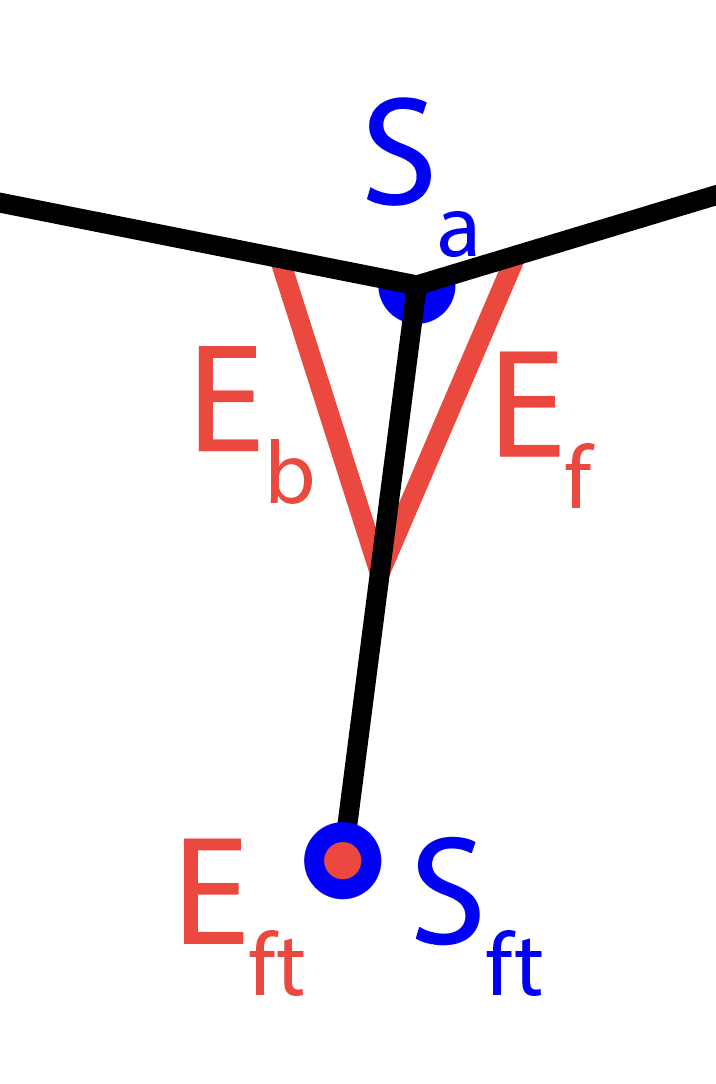
\includegraphics[width=\textwidth]{../plots/leg.png}
    \caption{}
    \label{fig:bodyPlot}
  \end{subfigure}%
  \begin{subfigure}[b]{0.29\textwidth}
    \vspace{0pt} % Adjust vertical spacing here
    \centering
    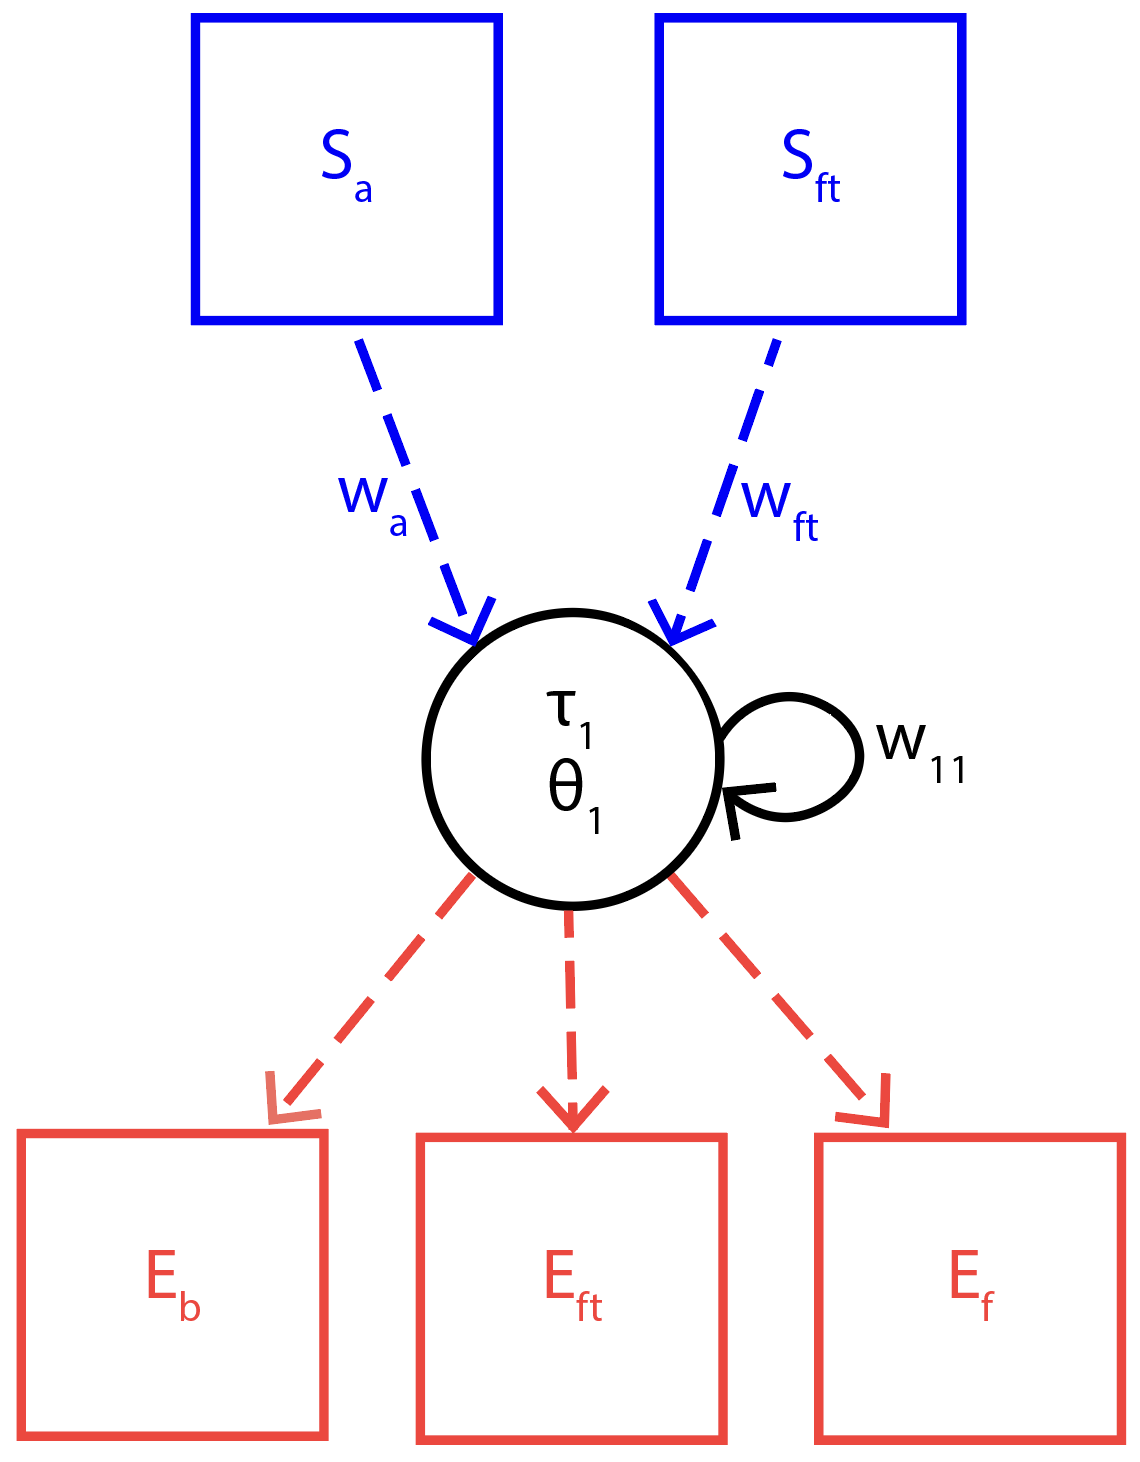
\includegraphics[width=\textwidth]{../plots/network1N.png}
    \caption{}
    \label{fig:N1Plot}
  \end{subfigure}%
  \begin{subfigure}[b]{0.41\textwidth}
    \vspace{0pt} % Adjust vertical spacing here
    \centering
    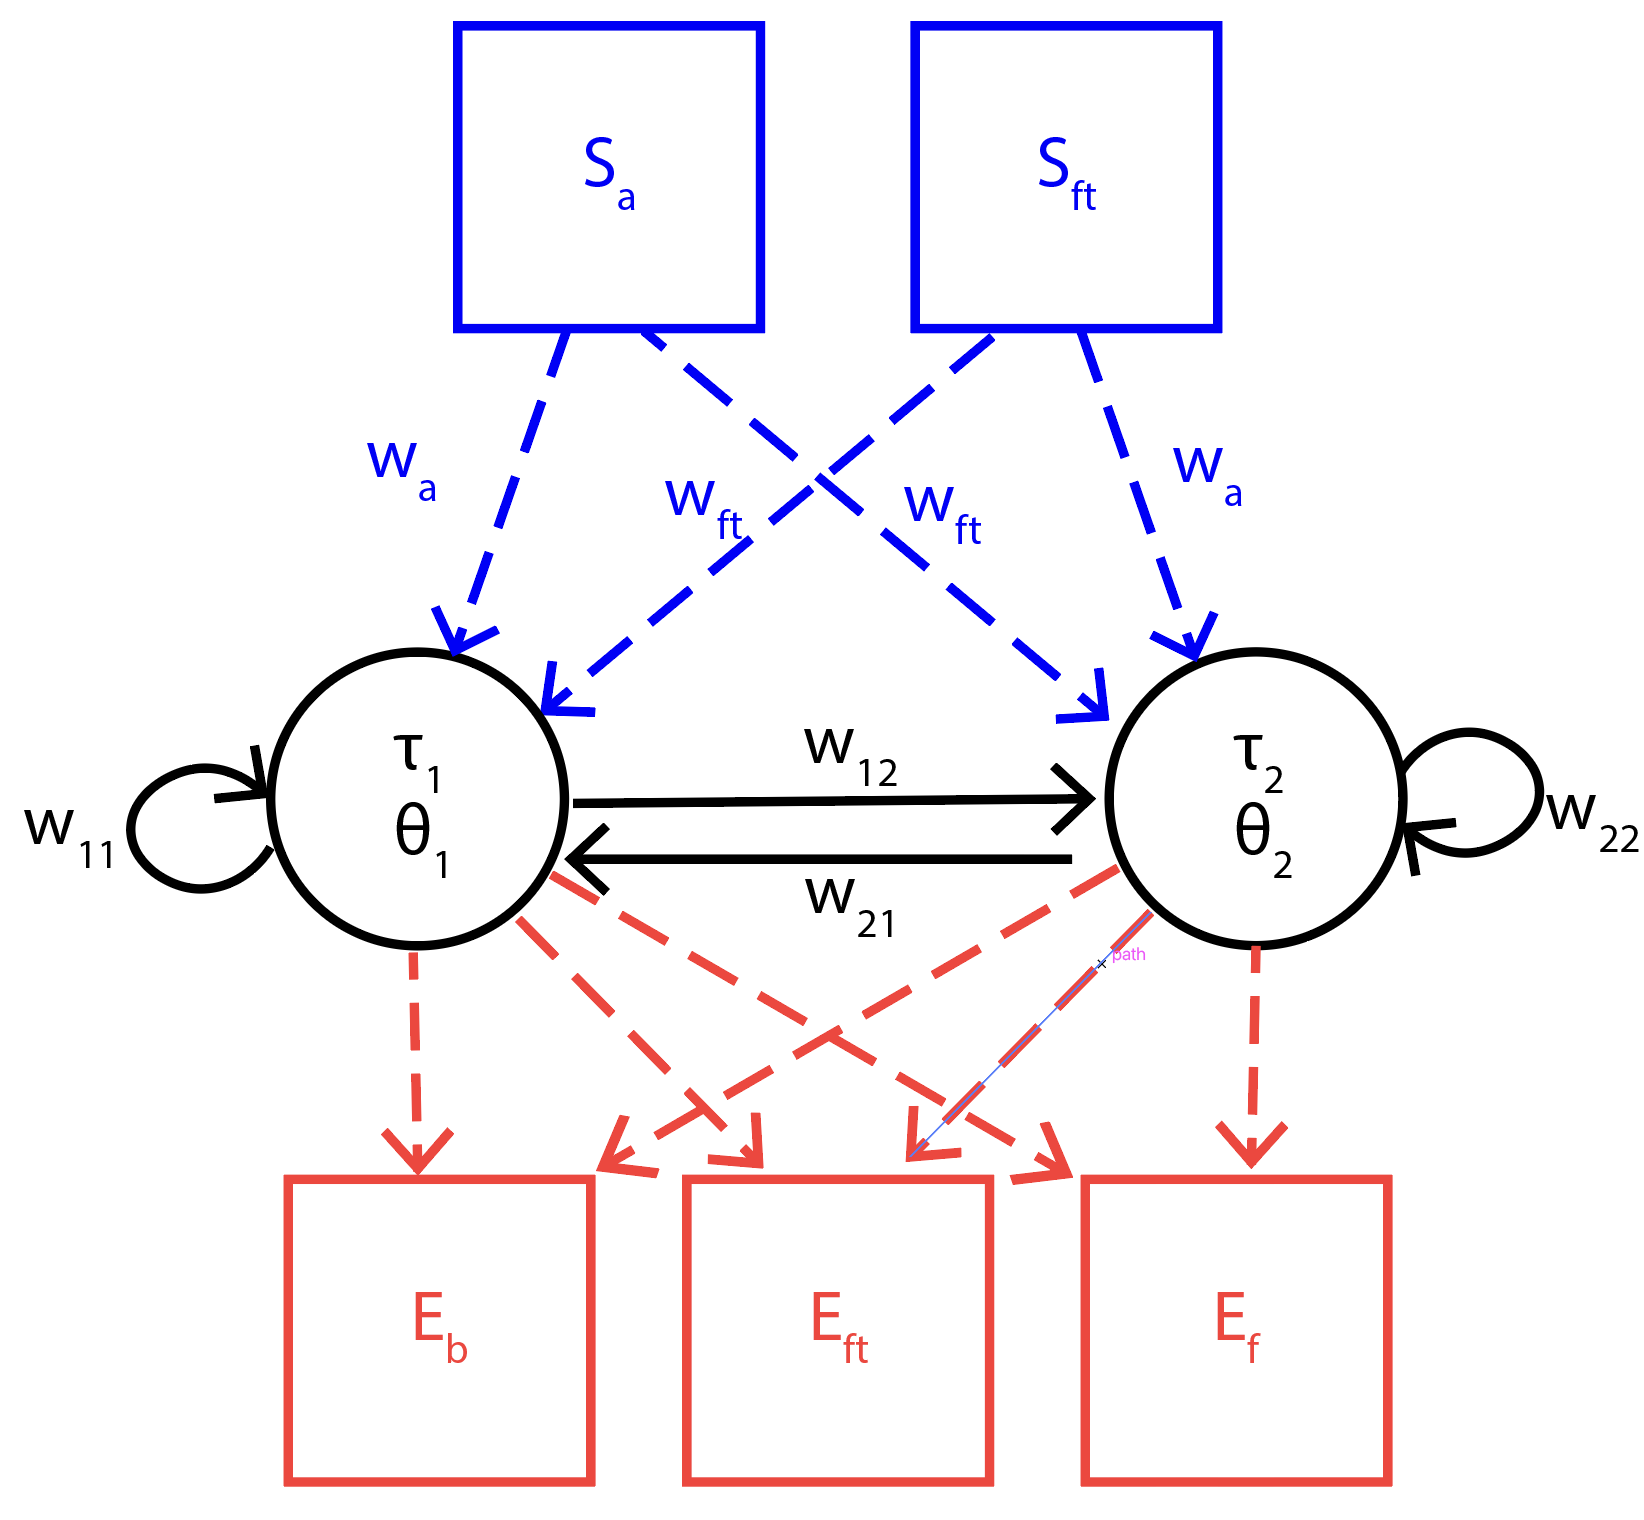
\includegraphics[width=\textwidth]{../plots/network2N.png}
    \caption{}
    \label{fig:N2Plot}
  \end{subfigure}
  \caption{(a) Diagram of agent body. Agent has two sensors, one for the leg angle $S_{a}$ and one for foot state $S_{ft}$. Anget has three effectors, one for forward swing $E_{f}$, one for backward swing $E_{b}$, and one for foot $E_{ft}$. (b) Network diagram of single neuron CTRNN. (c) Network diagram of two neuron CTRNN.}
  \label{fig:NetPlot}
\end{figure}

\subsection{Experimental Setup} The experiment involved evolving Continuous Time Recurrent Neural Networks (CTRNNs) with one and two neurons to control a single-legged walker, inspired by Beer \& Gallagher's 1992 model \cite{BeerWalker}. The output of each neuron is defined as:

\begin{equation}
  \dot{o}_i = \frac{1}{\tau_i} o_i(1 - o_i)\left(\sum_{j=1}^{N} w_{ji}o_j - \sigma^{-1}(o_i) + \theta_i + I_i \right) \quad i = 1, \dots, N.
\end{equation}

For this experiment, I evolved CTRNNs with one and two neurons. The CTRNNs controlled a single-legged walker with 3 effectors: a foot effector, a forward swing effector, and a backward swing effector. The foot effector controlled the state of the foot, which could be either in contact with the ground or not in contact with the ground. The forward swing effector controlled the forward swing of the leg, and the backward swing effector controlled the backward swing of the leg. The leg could swing forward or backward, but could not swing outside an angle range of \(\pi/6\) to -1 radians. If the leg reaches an angle of -1 radians, the leg angle will snap back to \(-\pi/6\) radians.

All \(3^{5N}\) possible sensorimotor configurations were tested for each number of neurons. A single evolutionary run was performed for each sensorimotor configuration, with the exception of redundant configurations. For example, the sensorimotor configuration [[1,1,1,1,1],[-1,-1,-1,-1,-1]] is redundant with the sensorimotor configuration [[-1,-1,-1,-1,-1],[1,1,1,1,1]], since the only difference between the two is the order of the neurons. 

The CTRNNs were evolved to control the leg of the walker to move forward as quickly as possible. The fitness of the networks was measured as the average velocity of the walker over 500 time steps with an integration step size of 0.1 time steps.

\subsection{Evolutionary Parameters and Network Design} The CTRNN parameters were evolved for each coupling combination, with variations in sensorimotor connections. All neurons could have incoming connections from the foot sensor and/or the angle sensor and outgoing connections to the foot effector, forward swing effector, and/or backward swing effector (see Fig \ref{fig:NetPlot}). These sensorimotor connections can be positive or negative. 
Each evolutionary run for one and two neuron CTRNNs lasted 10,000 generations. The one neuron runs had a population of 5000, and the two neuron runs had a population of 1000. Mutation variance was set at 0.2, and elitism at 0.05. The time constants \(\tau\) ranged from 1.0 to 10.0, with weights \(w\) and biases \(\phi\) ranging from -8.0 to 8.0. The weights \(w_a and w_{ft}\) of sensory connections ranged from 1.0 to 8.0. Gain was defaulted to 1.0 and was not changed over evolution. Each neuron had a self-connection and a connection to the other neuron in the case of the two neuron CTRNN.




For any neuron(s) connected to a sensor, the value of input was calculated by the following equations:
\begin{equation}
o_{S_{a}} = w_a \cdot \frac{ \phi  }{ \phi_{max} }
\end{equation}

\begin{equation}
o_{S_{ft}} = 
\begin{cases} 
0 & \text{for } o_{{E}_{ft}} = 0 \\
w_{ft} & \text{for } o_{{E}_{ft}} = 1
\end{cases}
\end{equation}

where \(o_{S_{a}}\) and \(o_{S_{ft}}\) are the outputs of the angle sensor and foot sensor, respectively, \(w_a\) and \(w_ft\) are their respective connection weights, \(\phi\) is the angle of the leg, \(\phi_{max}\) is the maximum angle of the leg (\(\pi/6\)), and \(o_{{E}_{ft}}\) is the output of the foot effector (i.e. the foot state). The state of the foot is 1 if the foot is in contact with the ground and 0 if the foot is not in contact with the ground.

Given these specifications for sensory output, the output of each neuron in the CTRNN can be more specifically defined as:

\begin{equation}
  \dot{o}_i = \frac{1}{\tau_i} o_i(1 - o_i)\left(\sum_{j=1}^{N} w_{ji}o_j - \sigma^{-1}(o_i) + \theta_i + I_i + w_{ai} o_{S_{a}} + w_{fti} o_{S_{ft}} \right) \quad \quad w_{ai}, w_{fti} \in \{-1, 0, 1\}, i = 1, \dots, N.
\end{equation}

where \(w_{ai}\) and \(w_{fti}\) are the connection weights from the angle sensor and foot sensor, respectively, to neuron \(i\). For any connections from a neuron to an effector, the output of the neuron is multiplied their connection weight, which is either 0 or ±1, and added to the effector.

\section{Results}
% Add your results content here

\subsection{One Neuron CTRNN}

\begin{figure}[htbp]
  \centering
  \begin{subfigure}[b]{0.5\textwidth}
    \vspace{0pt} % Adjust vertical spacing here
    \centering
    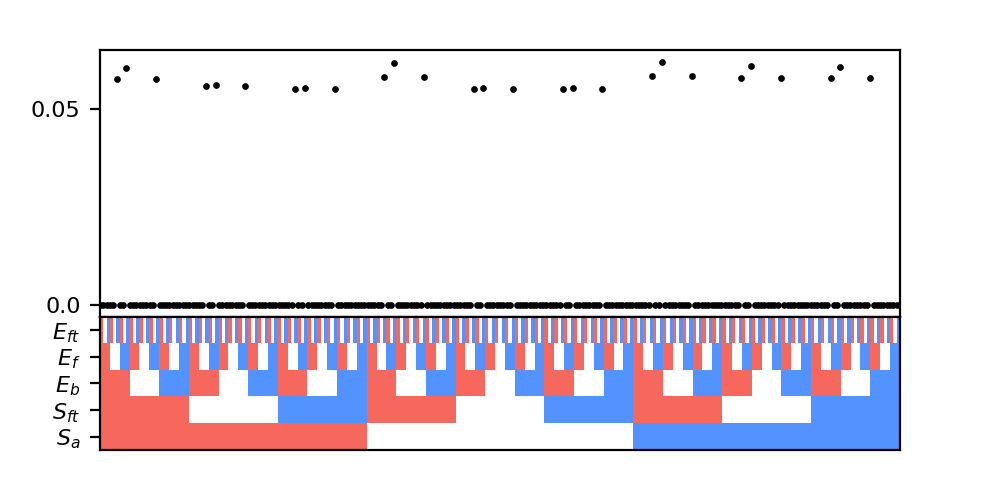
\includegraphics[width=\textwidth]{../plots/scatter1.png}
    \caption{}
    \label{fig:scatterPlot1A}
  \end{subfigure}%
  \hspace{-15pt}% Adjust horizontal spacing here
  \begin{subfigure}[b]{0.5\textwidth}
    \vspace{0pt} % Adjust vertical spacing here
    \centering
    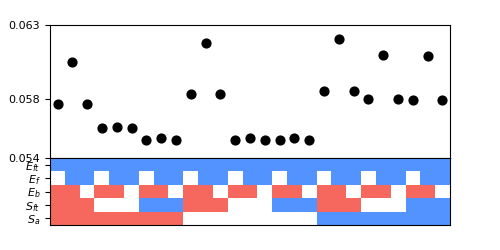
\includegraphics[width=\textwidth]{../plots/scatter1Working.png}
    \caption{}
    \label{fig:scatterPlot1B}
  \end{subfigure}
  \caption{(a) Best fitness of every one neuron CTRNN sensorimotor configuration. Each sensorimotor connection can be negative (red), 0 (white), or positive (blue). (b) Best fitness of every one neuron CTRNN sensorimotor configuration that was capable of movement.}
  \label{fig:scatterPlots1}
\end{figure}

\subsubsection{Fitness}
Evolution of all \(3^5\) (243) possible sensorimotor configurations of one neuron CTRNNs resulted in the majority of possible combinations being incapable of movement (see Fig \ref{fig:scatterPlot1A}). A mere 27 combinations resulted in a fitness of more than 0 (see Fig \ref{fig:scatterPlot1B}). The highest fitness of any agent was ~0.062, which translates to a maximum total distance of 31. Beer, Chiel, \& Gallagher found a single optimal step to cover a distance of 27.5 \cite{BeerOptimal}. Thus, even the best walker is not anywhere close to an optimal walker. Given that previous single neuron work exhibiting Reflexive Pattern Generators required the differential equations of the system to change dependent on the state of the foot effector, it is not surprising that a single neuron system with a single differential equation determining the output of the neuron would not be capable of generating such patterns \cite{BeerRPG}. 

\subsubsection{Connectivity}

Further examination of the sensorimotor configurations capable of movement reveals several patterns (see Fig \ref{fig:scatterPlot1B}). All of these configurations had a positive connection with the foot effector. Considering that the foot effector was activated when receiving a total signal of \(\geq 0.5\), this necessity is expected. Another necessary requirement to move was having a positive connection with the forward swing effector and/or a negative connection with the backward swing effector. Having both consistently led to the greatest overall fitness. A negative backward effector and a positive forward effector connection resulted in the same outcome, which explains why there was no noticeable difference in fitness between the two configurations. Any other effector combination would result in the walker attempting to move backward or not at all. 
The sensory connections were not essential for the walker to move but did affect fitness. Having a positive angle sensory connection and/or a negative foot sensory connection appeared to improve fitness.  
It also appears that a negative angle sensor connection may improve fitness, but only when there is no connection to the foot sensor (see columns 4-6 in Fig \ref{fig:scatterPlot1B}). It is not entirely clear why this is the case. Otherwise, a positive or neutral foot sensor connection did not have an impact on fitness.

\begin{figure}[htbp]
  \centering
  \begin{subfigure}[b]{0.32\textwidth}
    \centering
    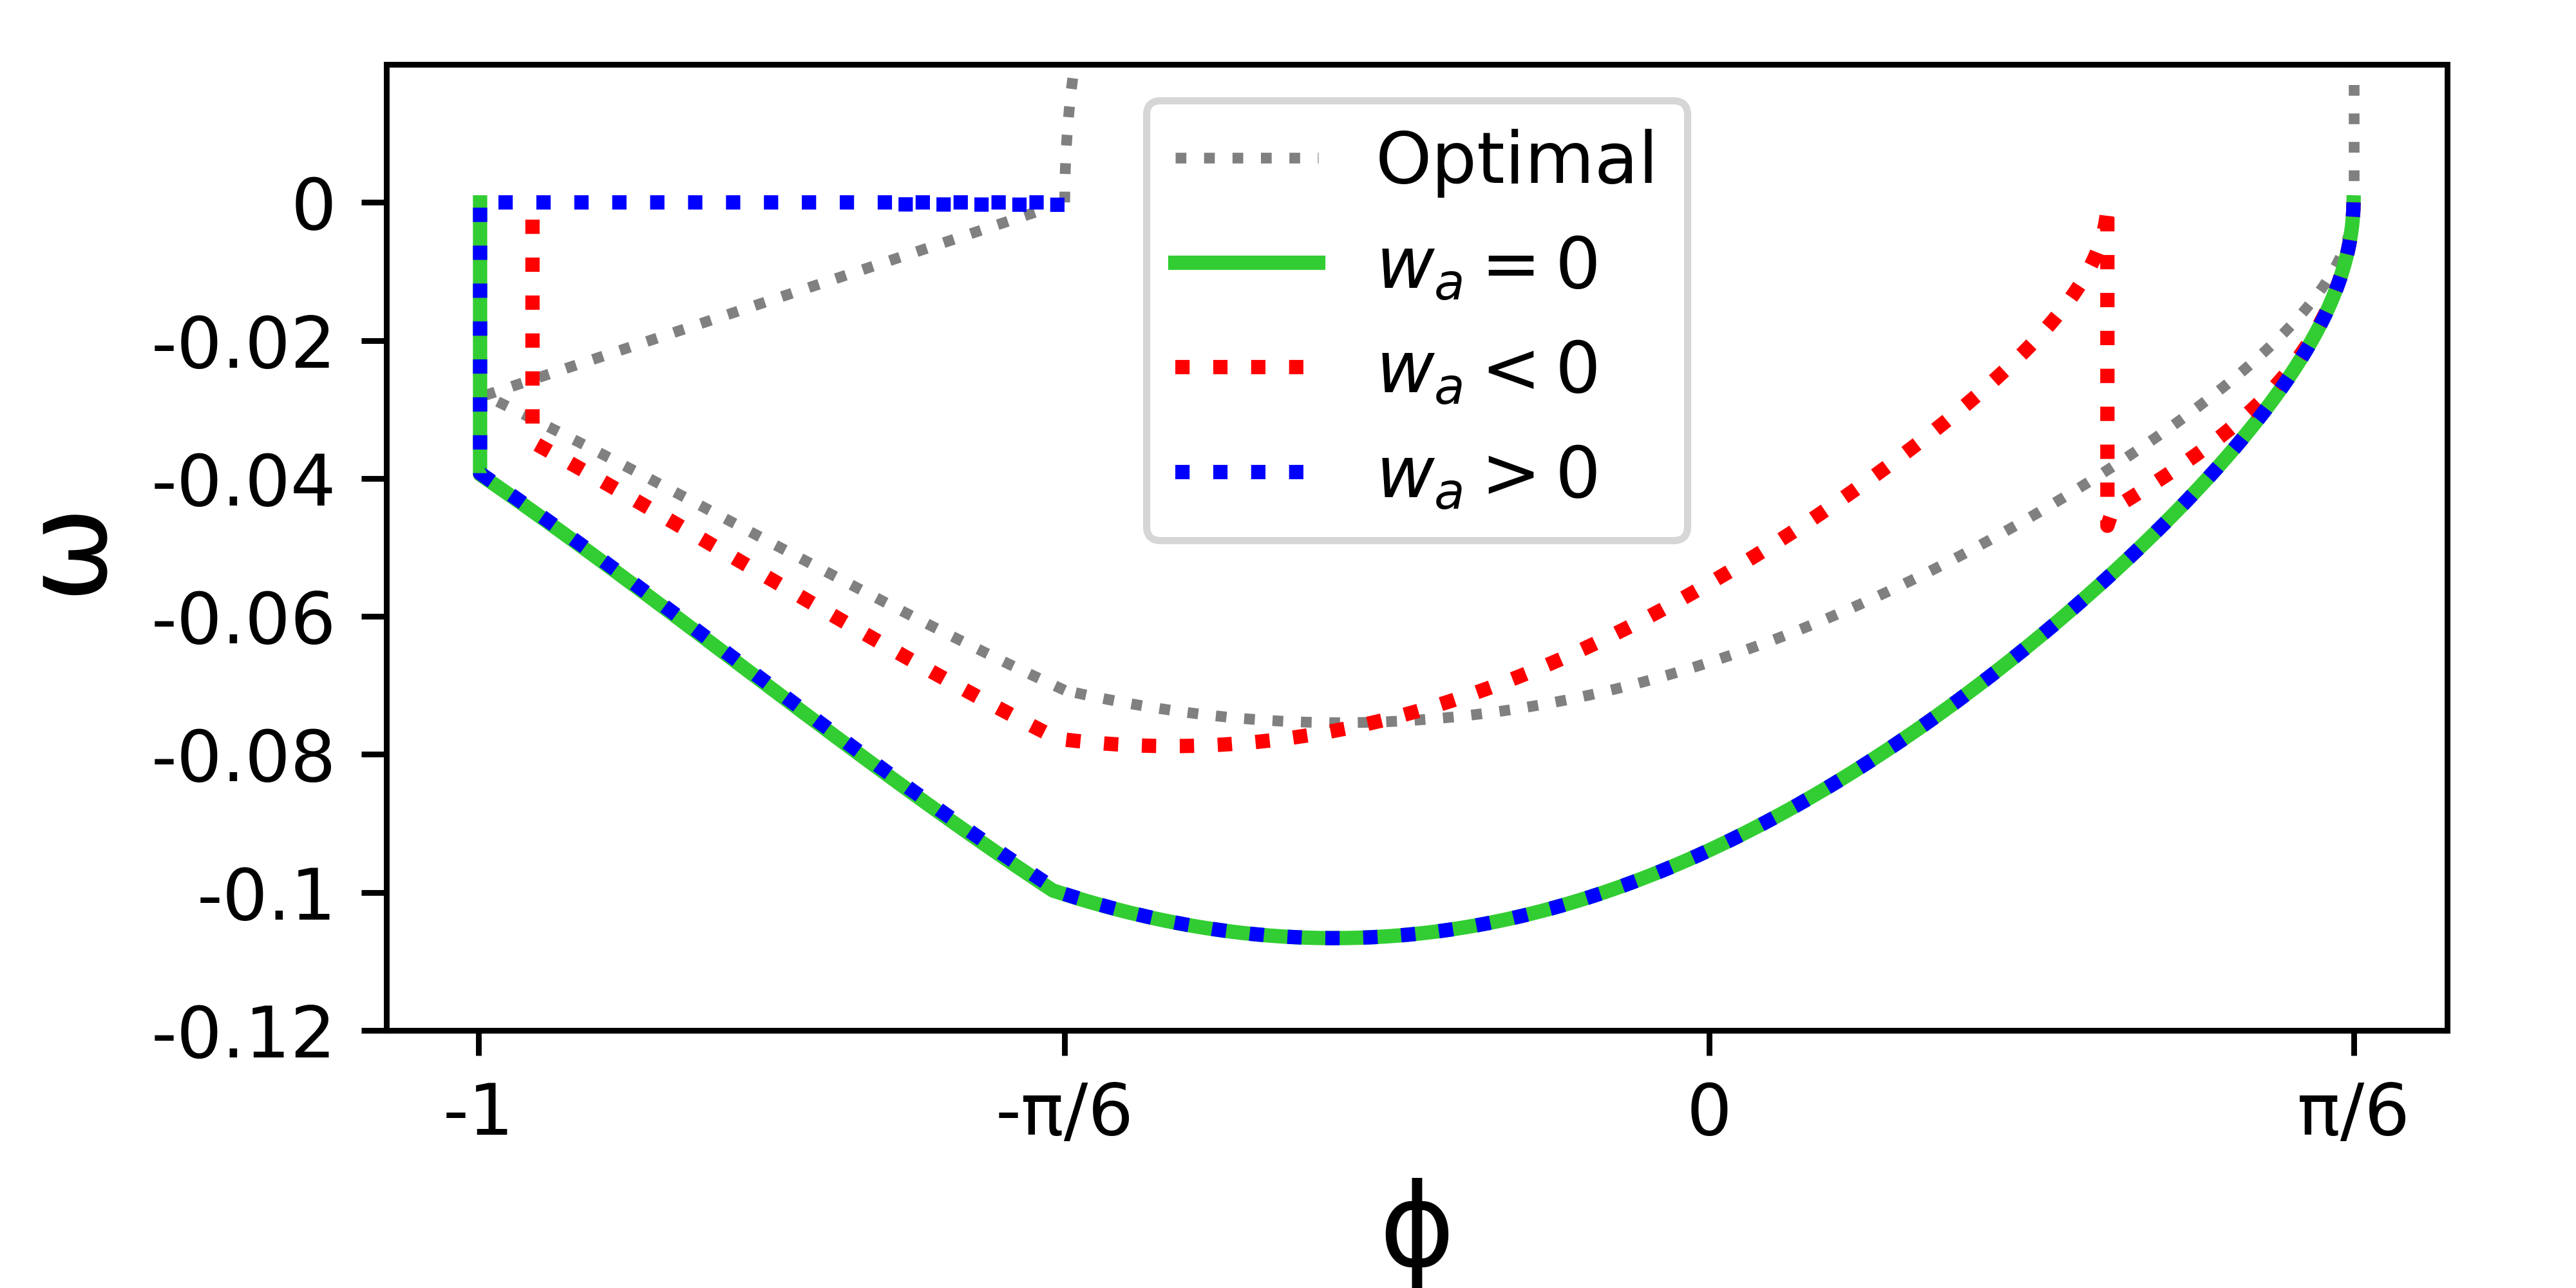
\includegraphics[width=\textwidth]{../plots/trajectory1comparison.png}
    \caption{}
    \label{fig:DuckPlot1Compare}
  \end{subfigure}
  % \hspace{-15pt}% Adjust horizontal spacing here
  \begin{subfigure}[b]{0.32\textwidth}
    \centering
    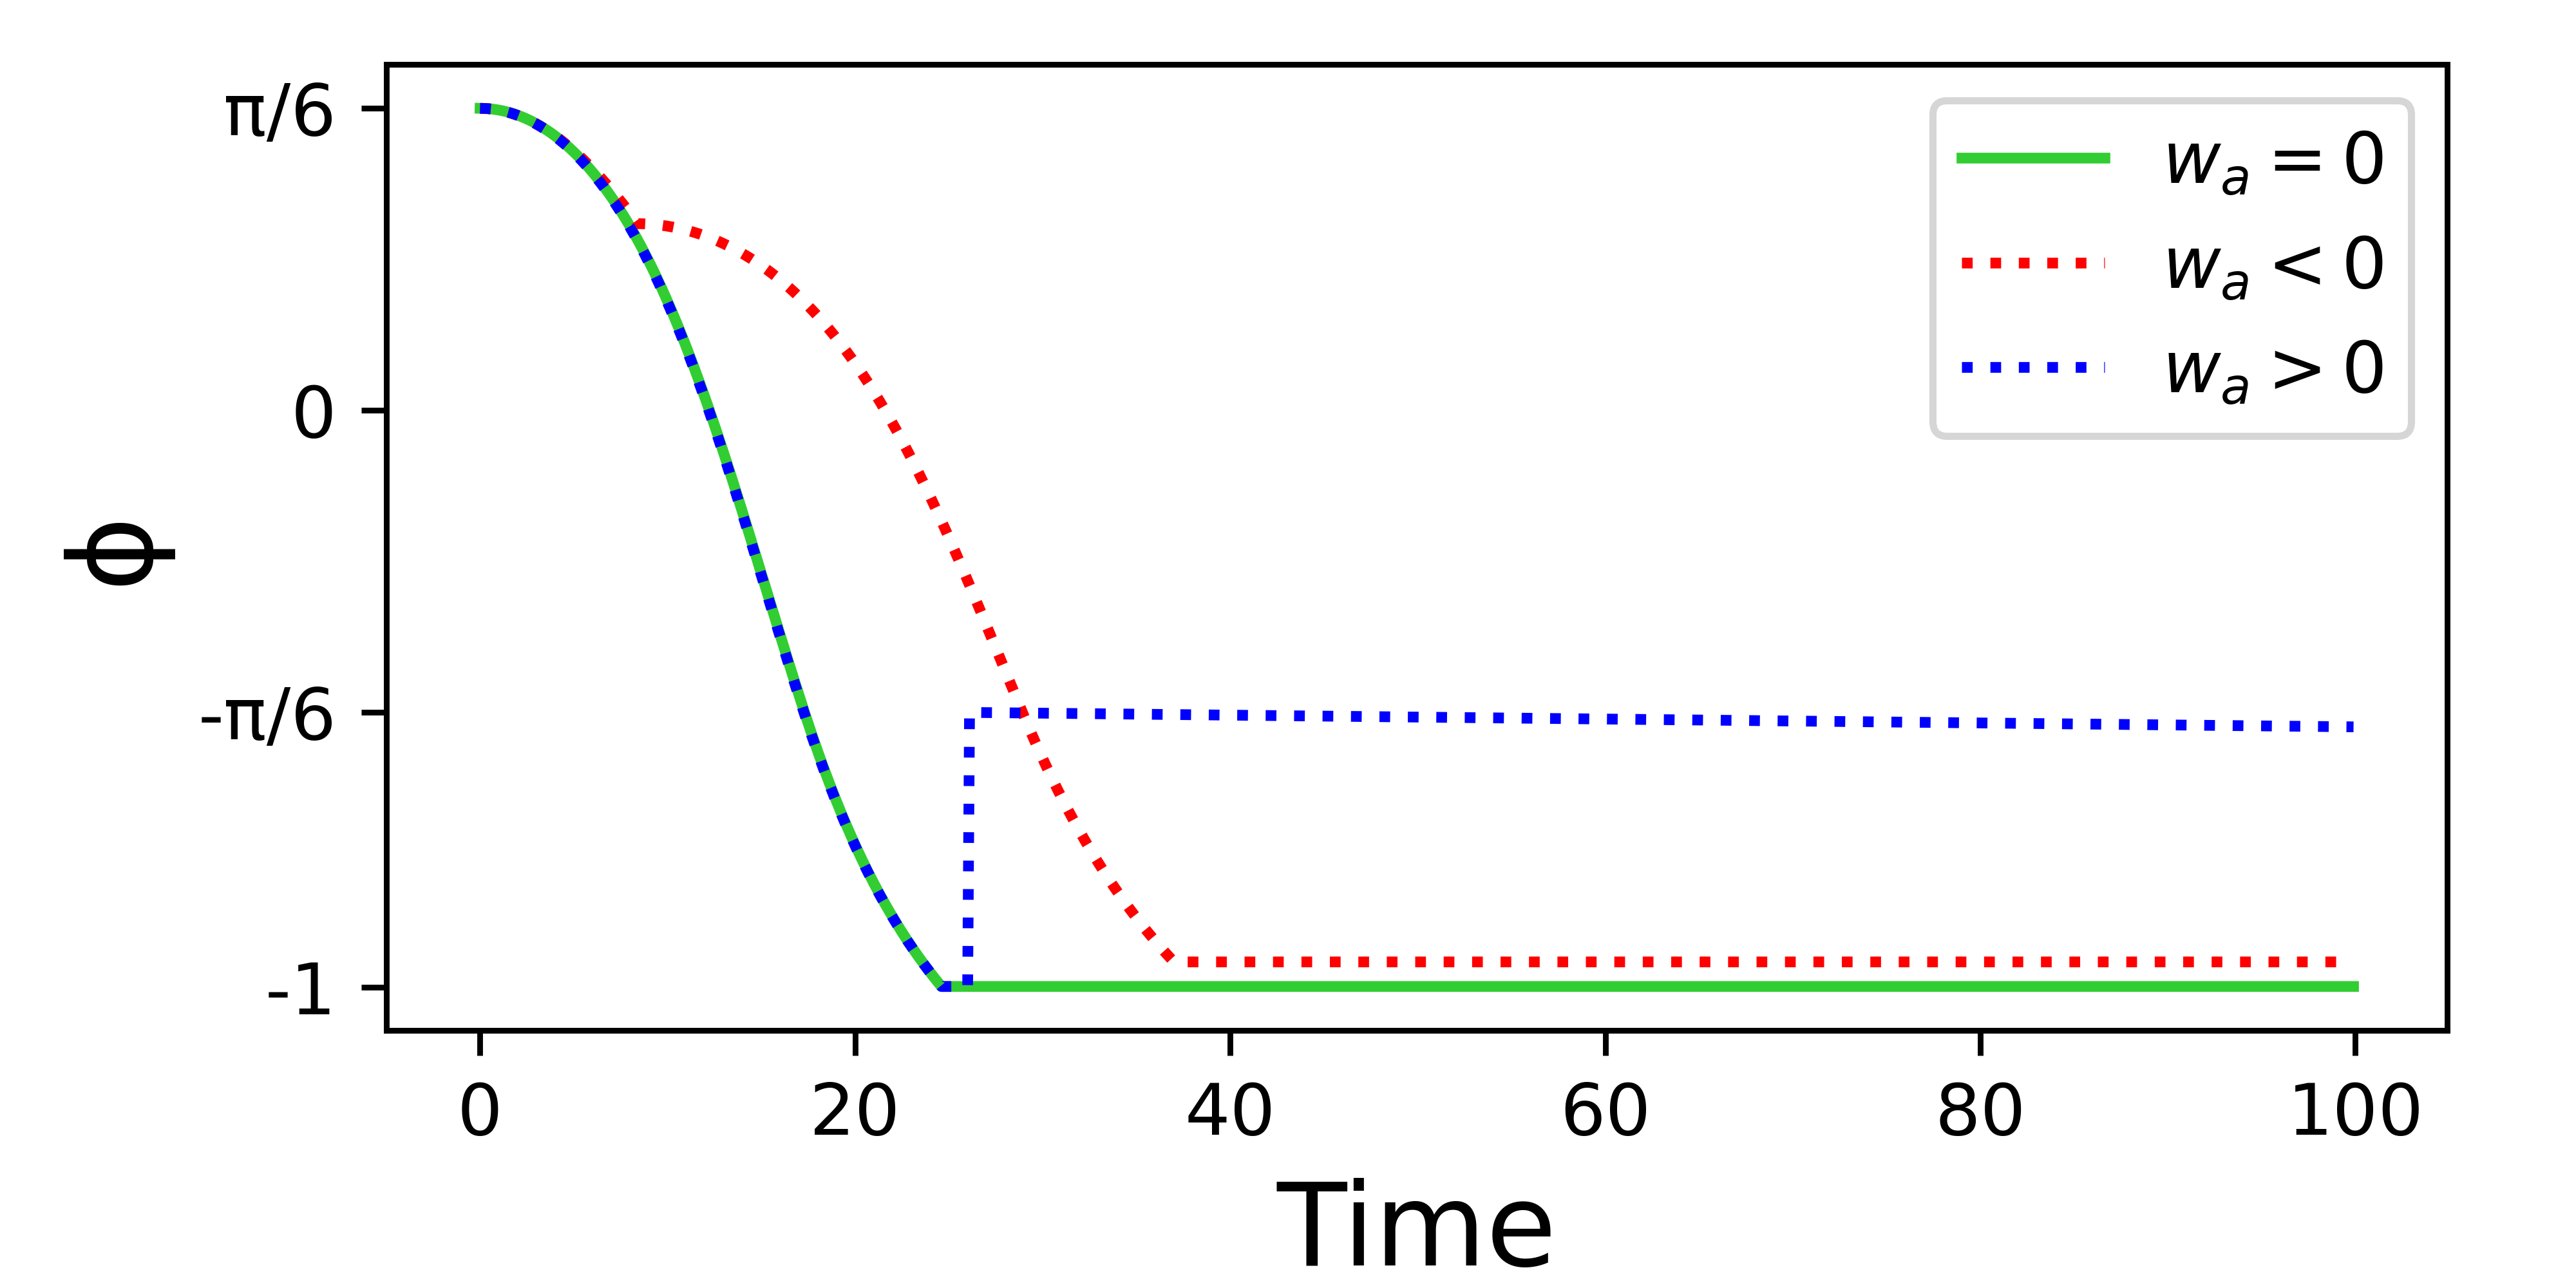
\includegraphics[width=\textwidth]{../plots/angleTime1comparison.png}
    \caption{}
    \label{fig:angleTimePlot1Compare}
  \end{subfigure}
  \begin{subfigure}[b]{0.32\textwidth}
    \centering
    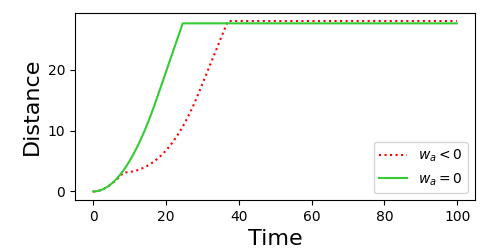
\includegraphics[width=\textwidth]{../plots/dist_compare.png}
    \caption{}
    \label{fig:distCompare}
  \end{subfigure}
  \caption{Plots of trajectories from agents with optimal effector connections [1,1,-1]. (a) Plot of leg trajectories as leg angle \((\phi)\) by leg angle velocity \((\omega)\), compared with optimal trajectory. (b) Plot of leg angles over time (c) Plot of distance over time for two of the agents.}
  \label{fig:comparePlots1}
\end{figure}

\subsubsection{Impact of Angle Sensory Connectivity on Behavior}

The angle sensor connection appears to have an impact on the overall fitness of the walker, but it is not clear how some agents received an increase to fitness from a negative connection to the angle sesnory only when there was no connection to the foot sensor. To better understand the impact of the angle sensor connection on the behavior of the walker, I examined the trajectories of the most fit agents with a negative angle sensor connection and no foot sensor connection [1,1,-1,0,?] (see Fig \ref{fig:comparePlots1}). The configuration with the positive angle sensory connection was the very close to the most fit configuration of [1,1,-1,-1,1] and shares an unusual behavior that improved its overall fitness, which we will examine in more depth later. It is the only configuration of the three shown to experience a "snapback" as a result of it hitting the negative leg angle limit of -1. The configuration with the neutral angle sensory connection was the least fit of the three, moving back its leg just shy of a leg angle of -1, stopping at -0.998702, just shy of the limit. Finally, the negative angle sensory connection configuration resulted in a fitness slightly higher than that from an agent with no sensory connection. At \(\phi \approx 0.323606 \) and \(\omega \approx -0.0468696\), the leg angle velocity is suddenly set to 0. As of now, I am not entirely sure why this is the case. As far as its improved fitness, this is also not clear. Given that the agent moves its leg back slightly less than the nonsensory agent (see Fig \ref{fig:angleTimePlot1Compare}), it is unexpected that the agent moves further than the nonsensory agent (see Fig \ref{fig:distCompare}). An potential explanation for this may be a result of a limitation with the precision in the floating point number calculations. Given that the negative connection agent takes a longer time to reach a similar distance, this could result in an accumulation of rounded values that ultimately result in a greater calculated distance. As it stands now, this phenomenon remains a mystery.

\subsubsection{Analysis of Most Fit Agent}

At first glance, the best performing agent, with a sensorimotor configuration of [1,1,-1,-1,1], does not perform very well at all (see Fig \ref{fig:angleTimePlot1Best}). As with all of the other single neuron CTRNNs, the agent is not able to switch into a swing phase after the "snapback" to \(-\pi/6\) from reaching the negative swing limit of -1, appearing to not move at all after this. However, if we examine its trajectory over a much longer time, it becomes apparent that the agent continues to move the leg backwards, using the snapback to oscillate the leg back and forth (see Fig \ref{fig:angleTimePlot1BestLong}). This oscillation results in the agent moving forward, albeit very slowly (see Fig \ref{fig:distPlot1Best}). This explains how this agent was capable of moving a distance greater than that of an optimal step.

\begin{figure}[htbp]
  \centering
  \begin{subfigure}[b]{0.32\textwidth}
    \centering
    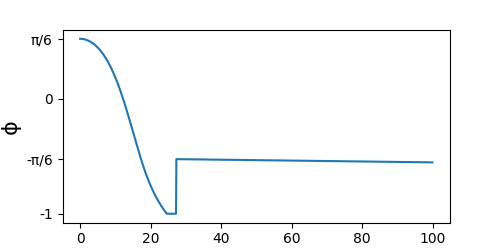
\includegraphics[width=\textwidth]{../plots/angleTime1_170.png}
    \caption{}
    \label{fig:angleTimePlot1Best}
  \end{subfigure}
  % \hspace{-15pt}% Adjust horizontal spacing here
  \begin{subfigure}[b]{0.32\textwidth}
    \centering
    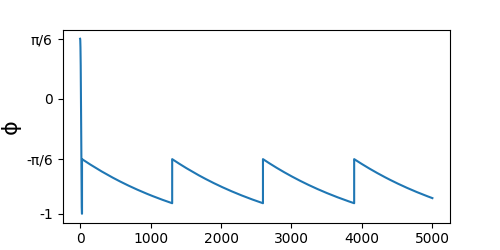
\includegraphics[width=\textwidth]{../plots/angleTime1_170_LONG.png}
    \caption{}
    \label{fig:angleTimePlot1BestLong}
  \end{subfigure}
  \begin{subfigure}[b]{0.32\textwidth}
    \centering
    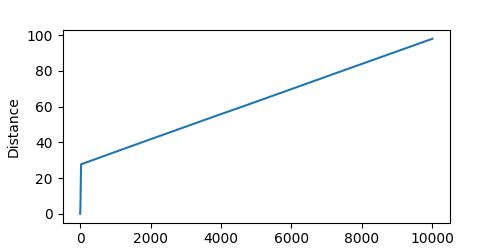
\includegraphics[width=\textwidth]{../plots/dist_170_LONG_X.png}
    \caption{}
    \label{fig:distPlot1Best}
  \end{subfigure}
  \caption{Plots of leg angle trajectories from most fit single-neuron agent [1,1,-1,-1,1]. (a) Plot of leg angles over time. (b) Plot of leg angles over time, with longer time scale. (c) Plot of distance over time.}
  \label{fig:angleTimePlots1Best}
\end{figure}

\subsection{Two Neuron CTRNN}  

\subsubsection{Fitness}
With \(3^{10}\) (59,049) possible sensorimotor configurations, the two neuron CTRNNs were capable of a much greater range of behaviors than the one neuron CTRNNs. The majority of possible combinations were still incapable of movement (see Fig \ref{fig:fitnessPlot2}). However, there were 8,235 possible combinations that were capable of movement, a slightly higher proportion than with the one neuron CTRNNs. The highest fitness of any agent was ~0.886, which is greater than the fitness of the "optimal" walker from Beer, Chiel, \& Gallagher \cite{BeerOptimal}.

\begin{figure}[htbp]
  \centering
  \begin{subfigure}[b]{0.5\textwidth}
    \vspace{0pt} % Adjust vertical spacing here
    \centering
    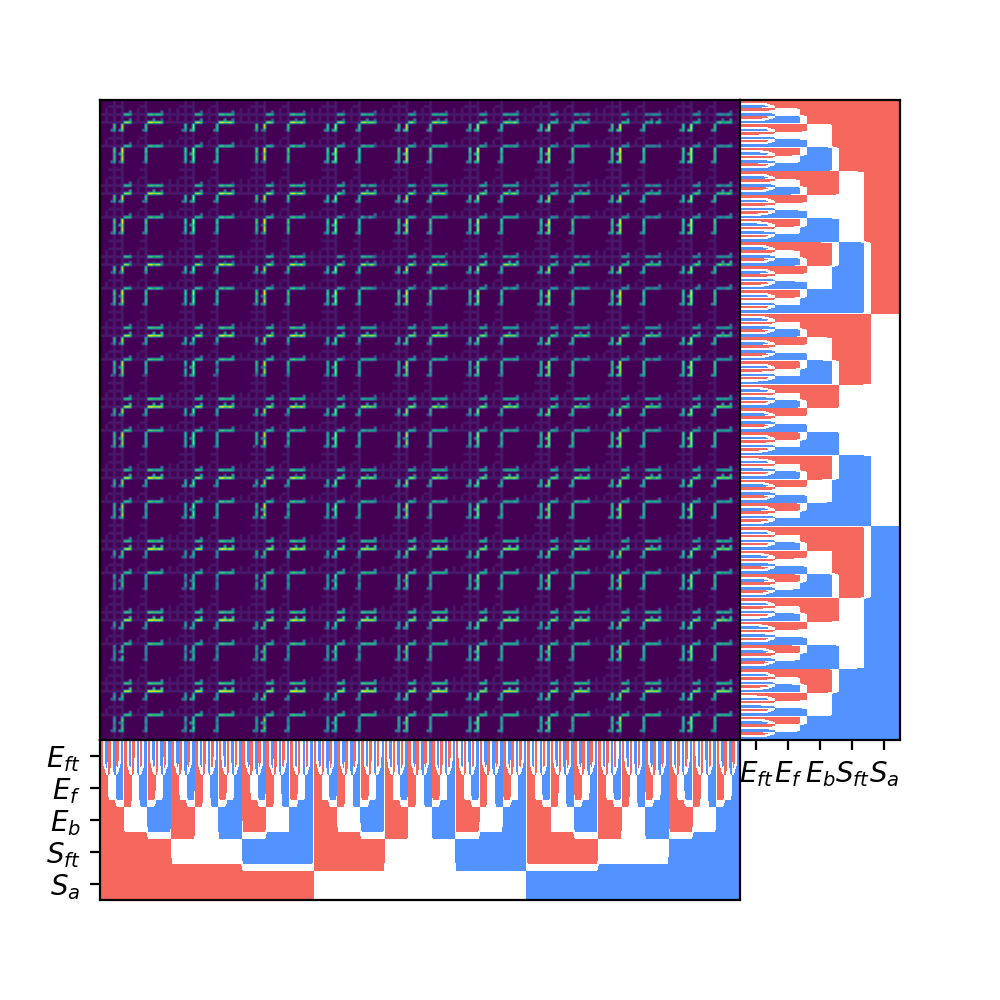
\includegraphics[width=\textwidth]{../plots/scatter2.png}
    \caption{}
    \label{fig:fitnessPlot2}
  \end{subfigure}%
  \hspace{-15pt}% Adjust horizontal spacing here
  \begin{subfigure}[b]{0.5\textwidth}
    \vspace{0pt} % Adjust vertical spacing here
    \centering
    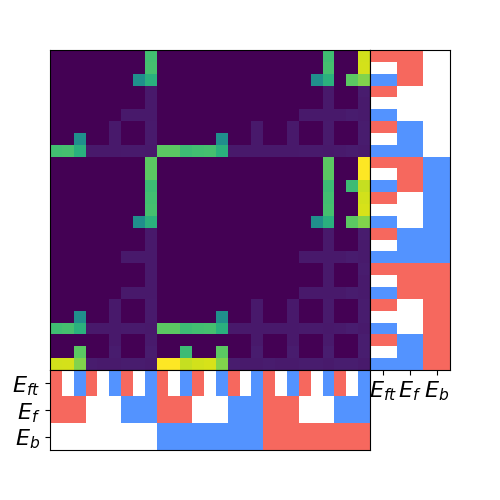
\includegraphics[width=\textwidth]{../plots/scatter2WorkingPattern.png}
    \caption{}
    \label{fig:fitnessPlot2Pattern}
  \end{subfigure}
  \caption{(a) Best fitness of every two neuron CTRNN sensorimotor configuration. Each sensorimotor connection can be negative (red), 0 (white), or positive (blue). (b) Best fitness of every two neuron CTRNN motor configuration. This pattern repeats over every sensory configuration.}
  \label{fig:fitnessPlots2}
\end{figure}

\subsubsection{Connectivity}
Like with the single neuron case, effector connectivity determined whether or not an agent was capable of any movement at all. Whether an agent was capable of movement could be defined by the following logical statement:

\begin{equation}
(w_{1ft} = 1 \vee w_{2ft} = 1)  \wedge ((w_{1f} - w_{1b} > -(w_{2f} - w_{2b})) \vee (w_{2f} - w_{2b} > -(w_{1f} - w_{1b}) )
\end{equation}

where \(w_{ift}\) is the weight of the connection from neuron \(i\) to effector \(E_{ft}\), \(w_{if}\) is the weight of the connection from neuron \(i\) to effector \(E_f\), and \(w_{ib}\) is the weight of the connection from neuron \(i\) to effector \(E_b\). The lowest $w_{ift}$ can be is $-1$ and, since \(1-1=0\), this can be simplified to:

\[\sum_{i=1}^{2} w_{ift} \geq 0 \ \wedge \ ((w_{1f} - w_{1b} > -(w_{2f} - w_{2b})) \vee (w_{2f} - w_{2b} > -(w_{1f} - w_{1b}) )\]

This can be further simplified to:

\[\sum_{i=1}^{2} w_{ift} \geq 0 \ \wedge \ ((w_{1f} - w_{1b} > w_{2b}- w_{2f}) \vee (w_{2f} - w_{2b} > w_{1b} - w_{1f}) )\]

\[\sum_{i=1}^{2} w_{ift} \geq 0 \ \wedge \ (w_{1f} + w_{2f} > w_{1b} + w_{2b}) \]

\[\sum_{i=1}^{2} w_{ift} \geq 0 \ \wedge \ \sum_{i=1}^{2} w_{if} > \sum_{i=1}^{2} w_{ib} \]

Given that the number of neurons ($N$) is 2 in this case, we can generalize the above statement to:

\begin{equation}
  \sum_{i=1}^{N} w_{ift} \geq 0 \ \wedge \ \sum_{i=1}^{N} w_{if} > \sum_{i=1}^{N} w_{ib}
\end{equation}

Meeting these conditions in a two neuron CTRNN was necessary and sufficient to produce movement. This logical statement also proves true for the one neuron CTRNN.

\begin{figure}[htbp]
  \centering
  \begin{subfigure}[b]{0.5\textwidth}
    \vspace{0pt} % Adjust vertical spacing here
    \centering
    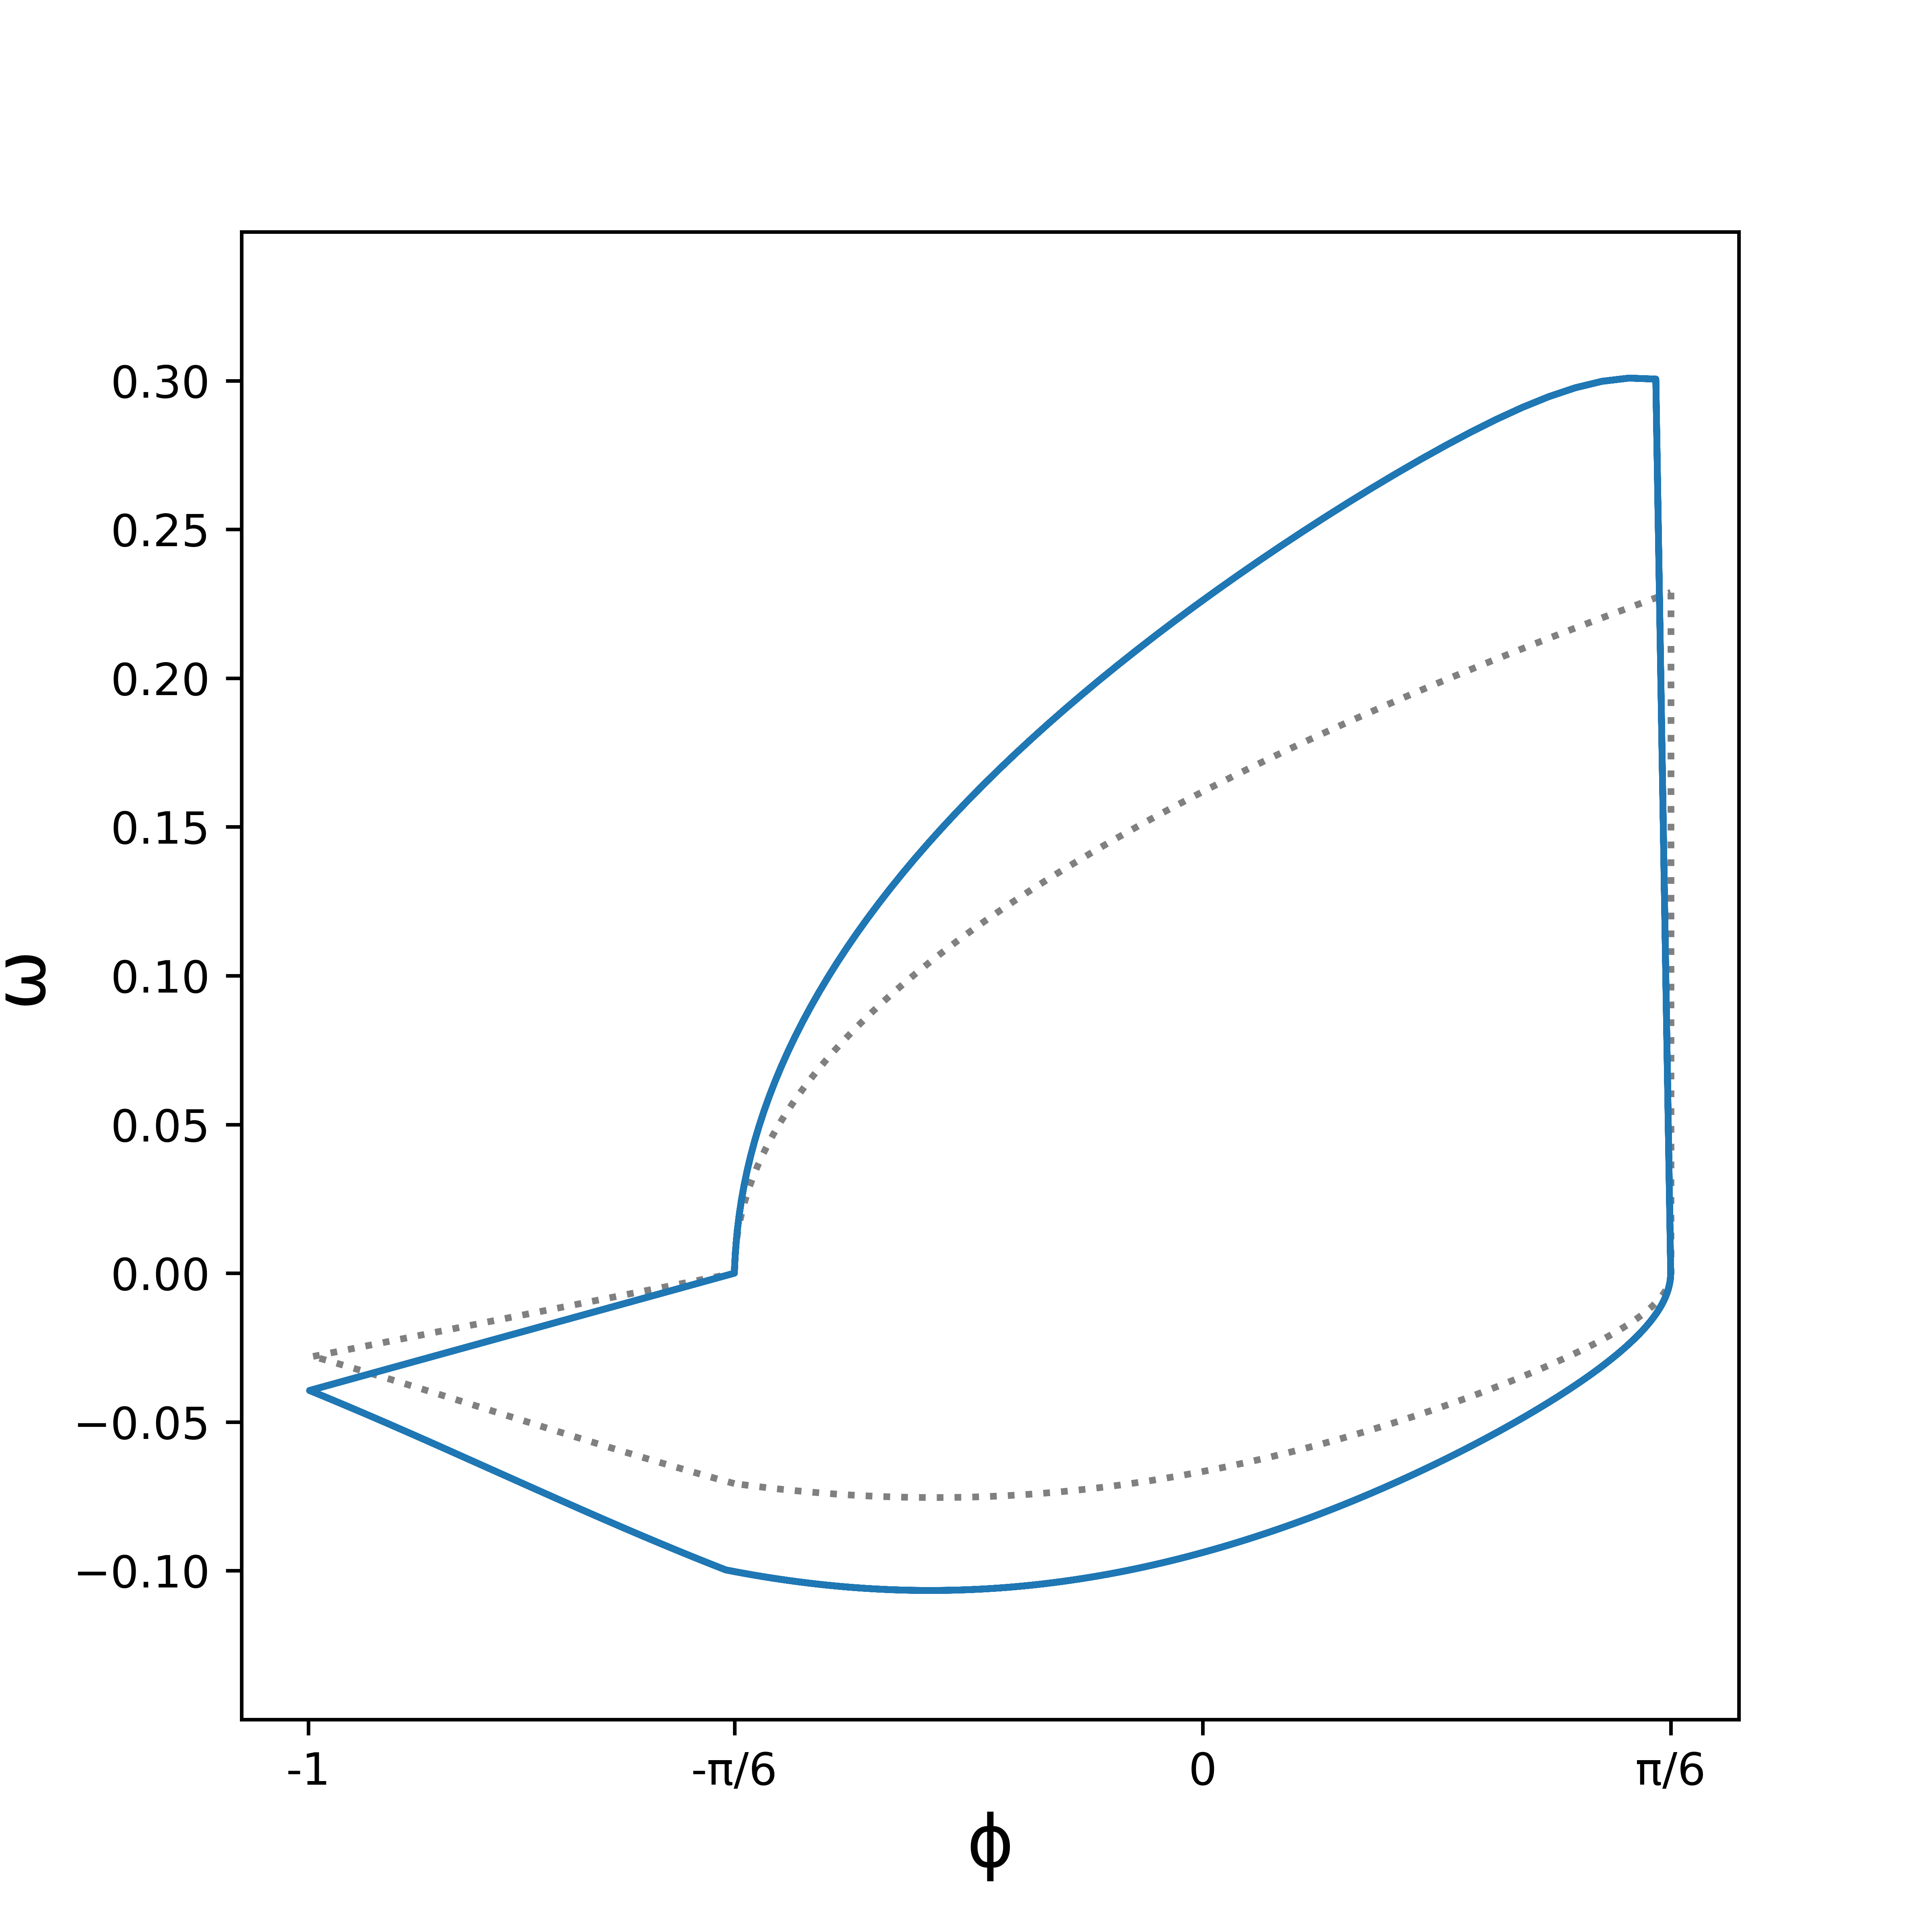
\includegraphics[width=\textwidth]{../plots/trajectory2_224_18.png}
    \caption{}
    \label{fig:DuckPlot2Best}
  \end{subfigure}%
  \hspace{-15pt}% Adjust horizontal spacing here
  \begin{subfigure}[b]{0.5\textwidth}
    \vspace{0pt} % Adjust vertical spacing here
    \centering
    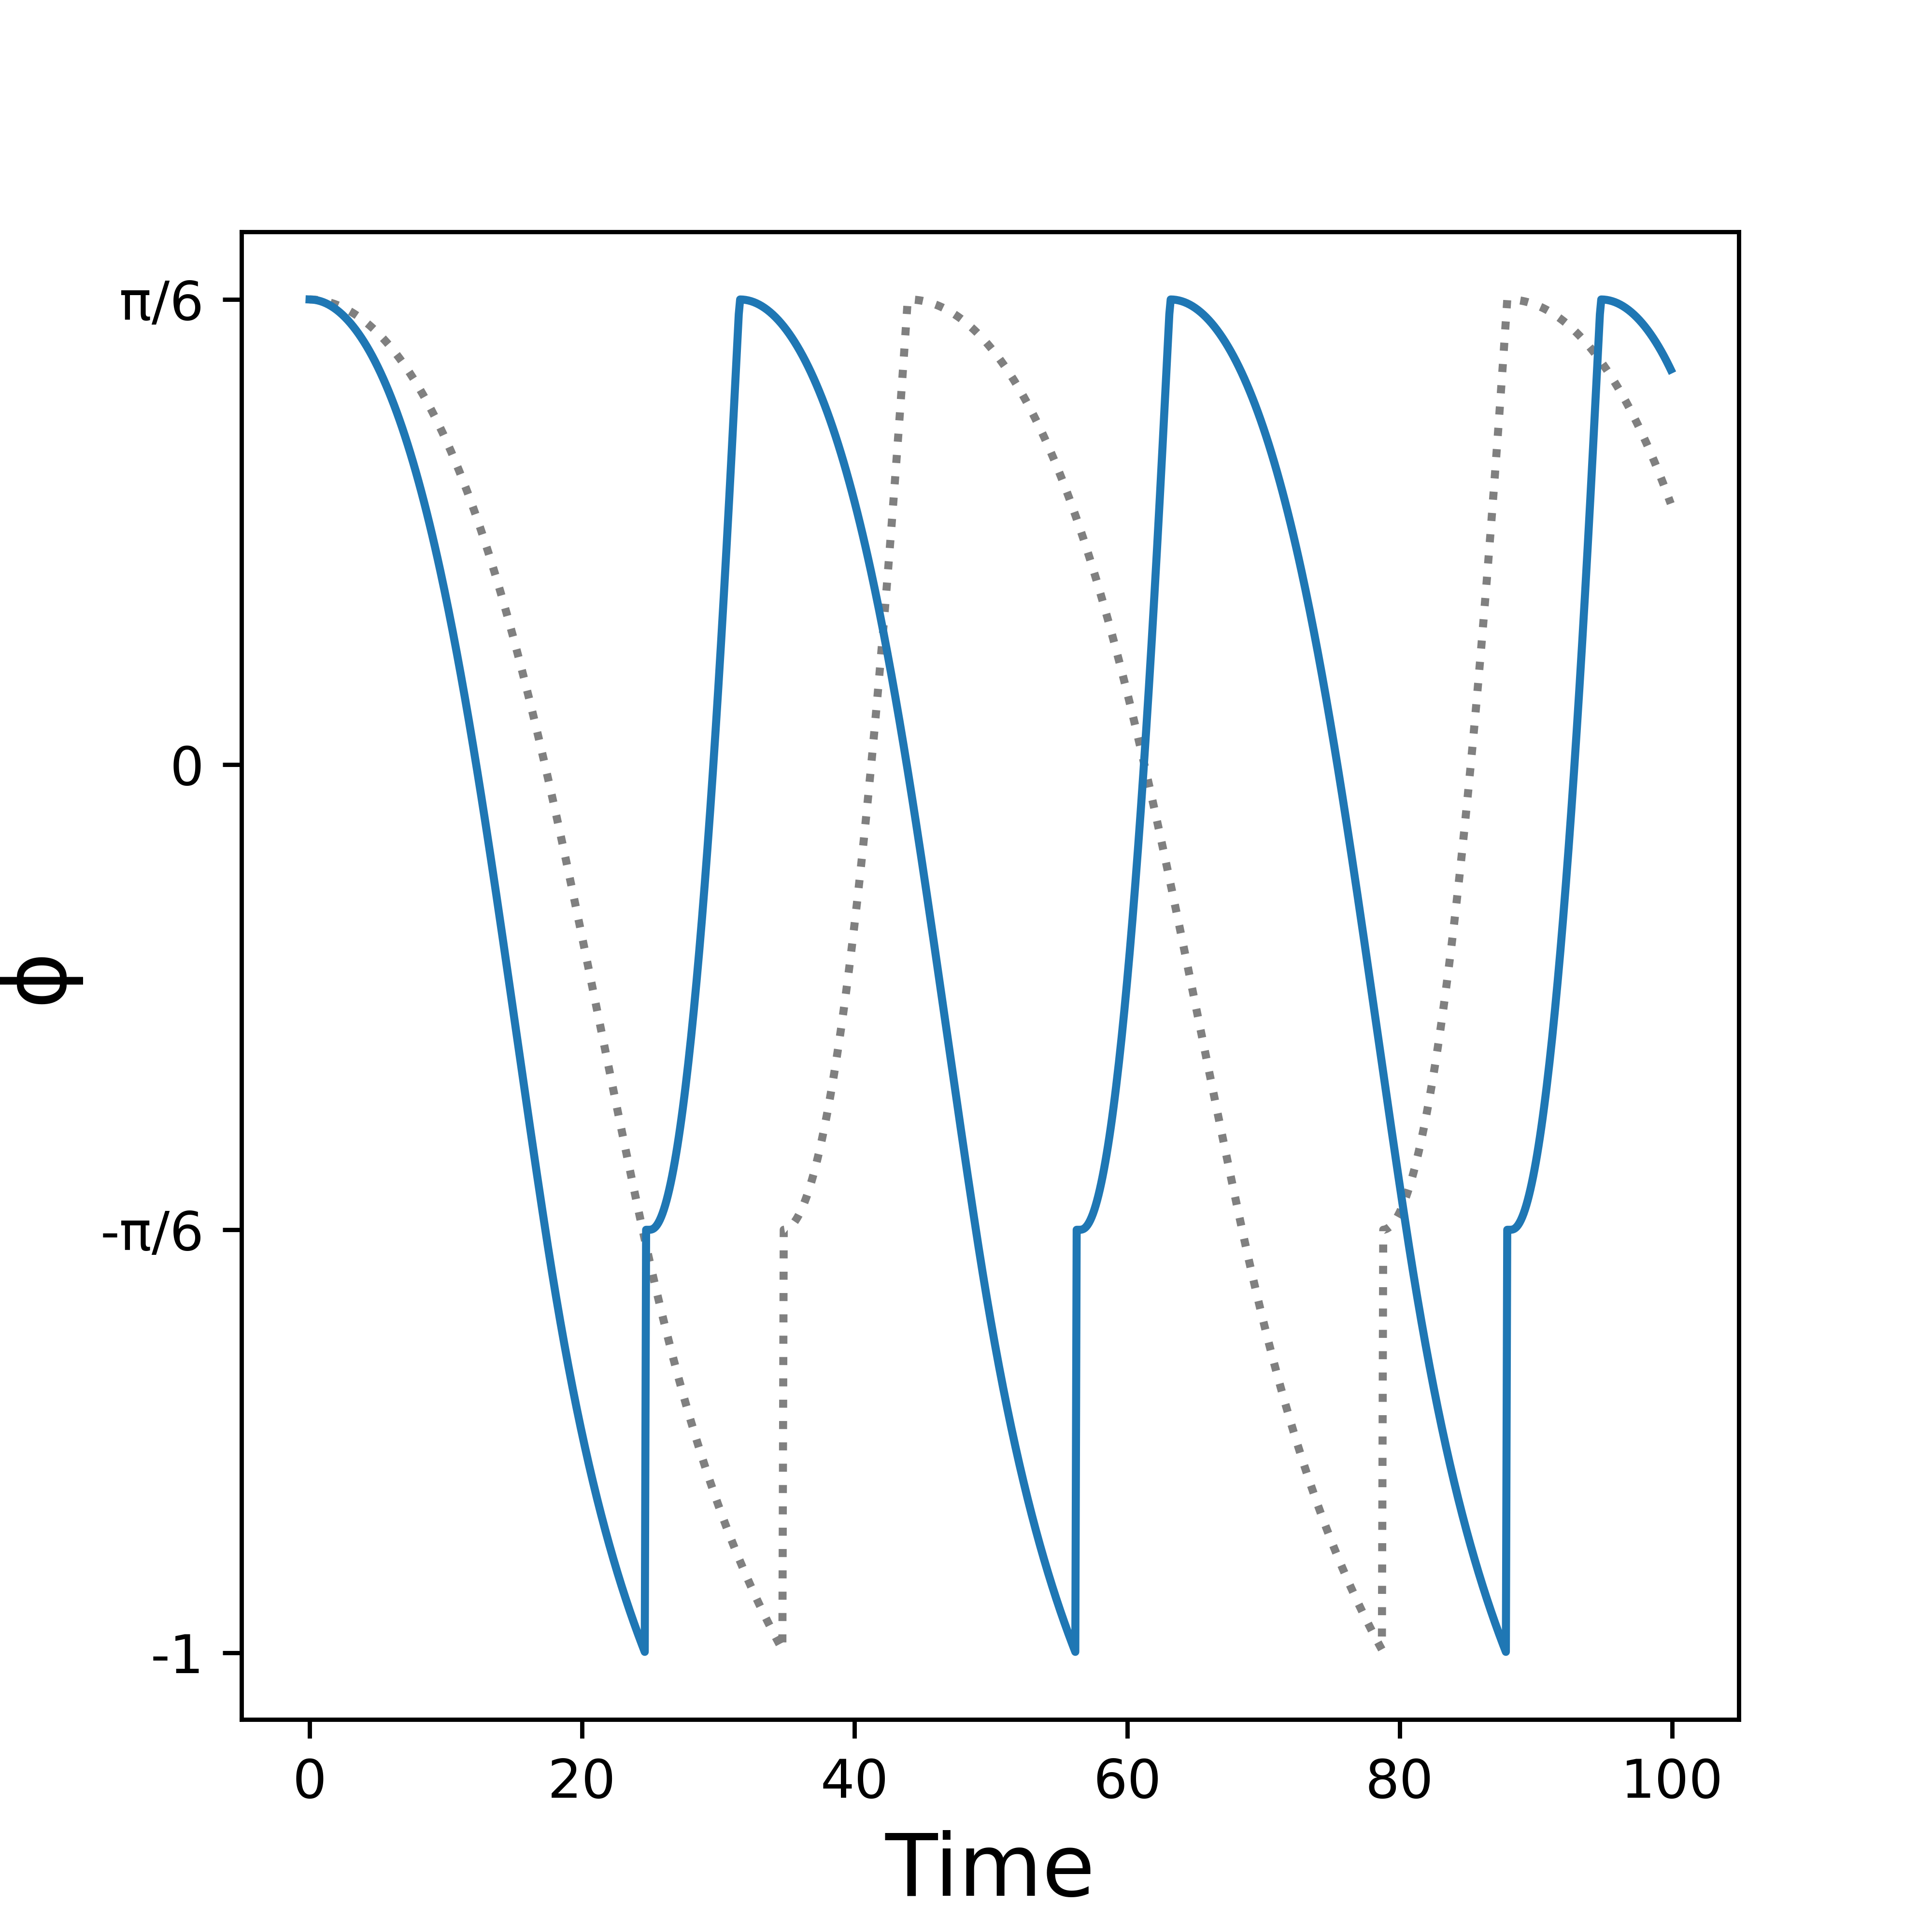
\includegraphics[width=\textwidth]{../plots/angleTime2_224_18.png}
    \caption{}
    \label{fig:AngleTimePlot2Best}
  \end{subfigure}
  \caption{Plots of trajectory of most fit two neuron agent [[1,1,-1,1,1],[-1,-1,1,-1,-1]] (blue) compared with optimal trajectory (grey). (a) Plot of leg trajectories as leg angle \((\phi)\) by leg angle velocity \((\omega)\). (b) Plot of leg angles over time}
  \label{fig:plots2Best}
\end{figure} 

\subsubsection{Analysis of Most Fit Agent}

With sensorimotor connectivity of [[1,1,-1,1,1],[-1,-1,1,-1,-1]], the most fit two neuron agent was capable of reaching a fitness of 0.886. Given that this is a much greater fitness than the optimal walker, this does not seem possible. Looking at the trajectory of the agent, how this agent is able to reach this fitness score becomes apparent (see Fig \ref{fig:plots2Best}). With each neuron able to output to two effectors each, the resulting output to the two effectors is much higher than it would be when each effector is limited to a single neuron each, resulting in a step that is the same overall distance as the optimal step but with a much higher velocity. 

\begin{figure}[htbp]
  \centering
  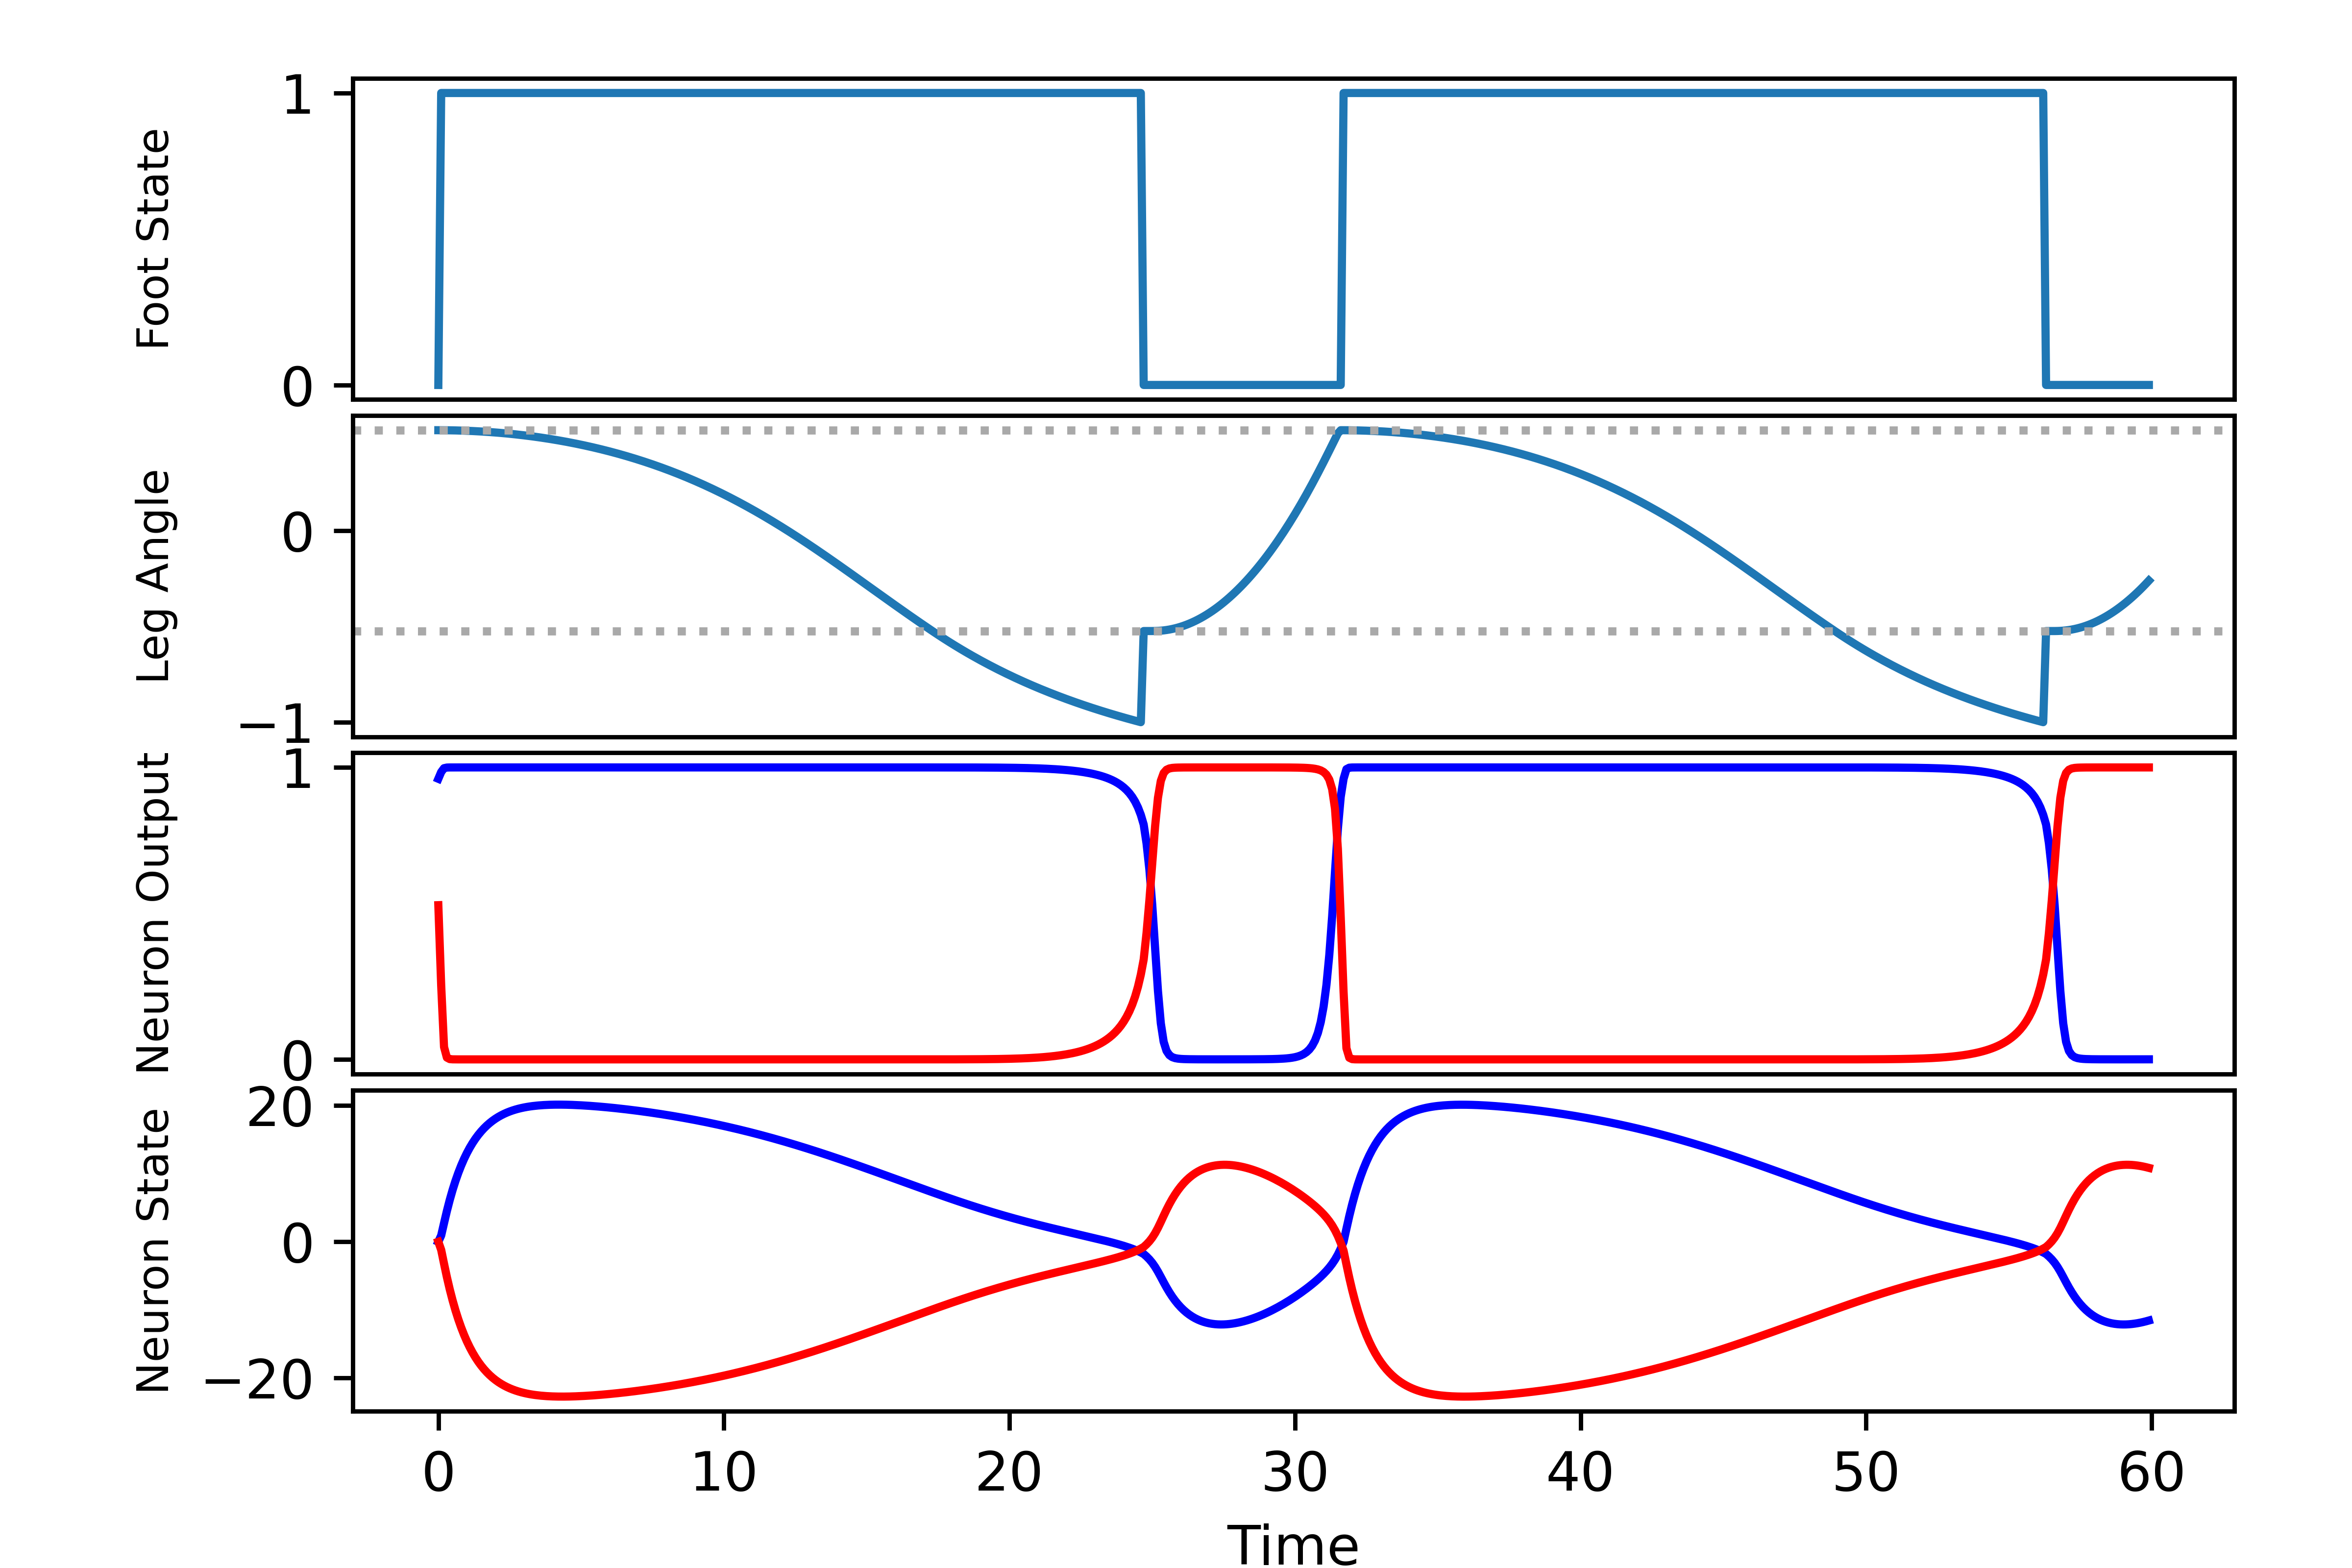
\includegraphics[width=.8\textwidth]{../plots/angleTime2_224_18_Foot.png}
  \caption{A plot of the foot state, leg angle, neural output, and neural state over time for the most fit two neuron agent. Neuron 1 is in blue, and neuron 2 is in red.}
  \label{fig:fullplot2Best}
\end{figure}

\begin{figure}[htbp]
  \centering
  \begin{subfigure}[b]{0.5\textwidth}
    \vspace{0pt} % Adjust vertical spacing here
    \centering
    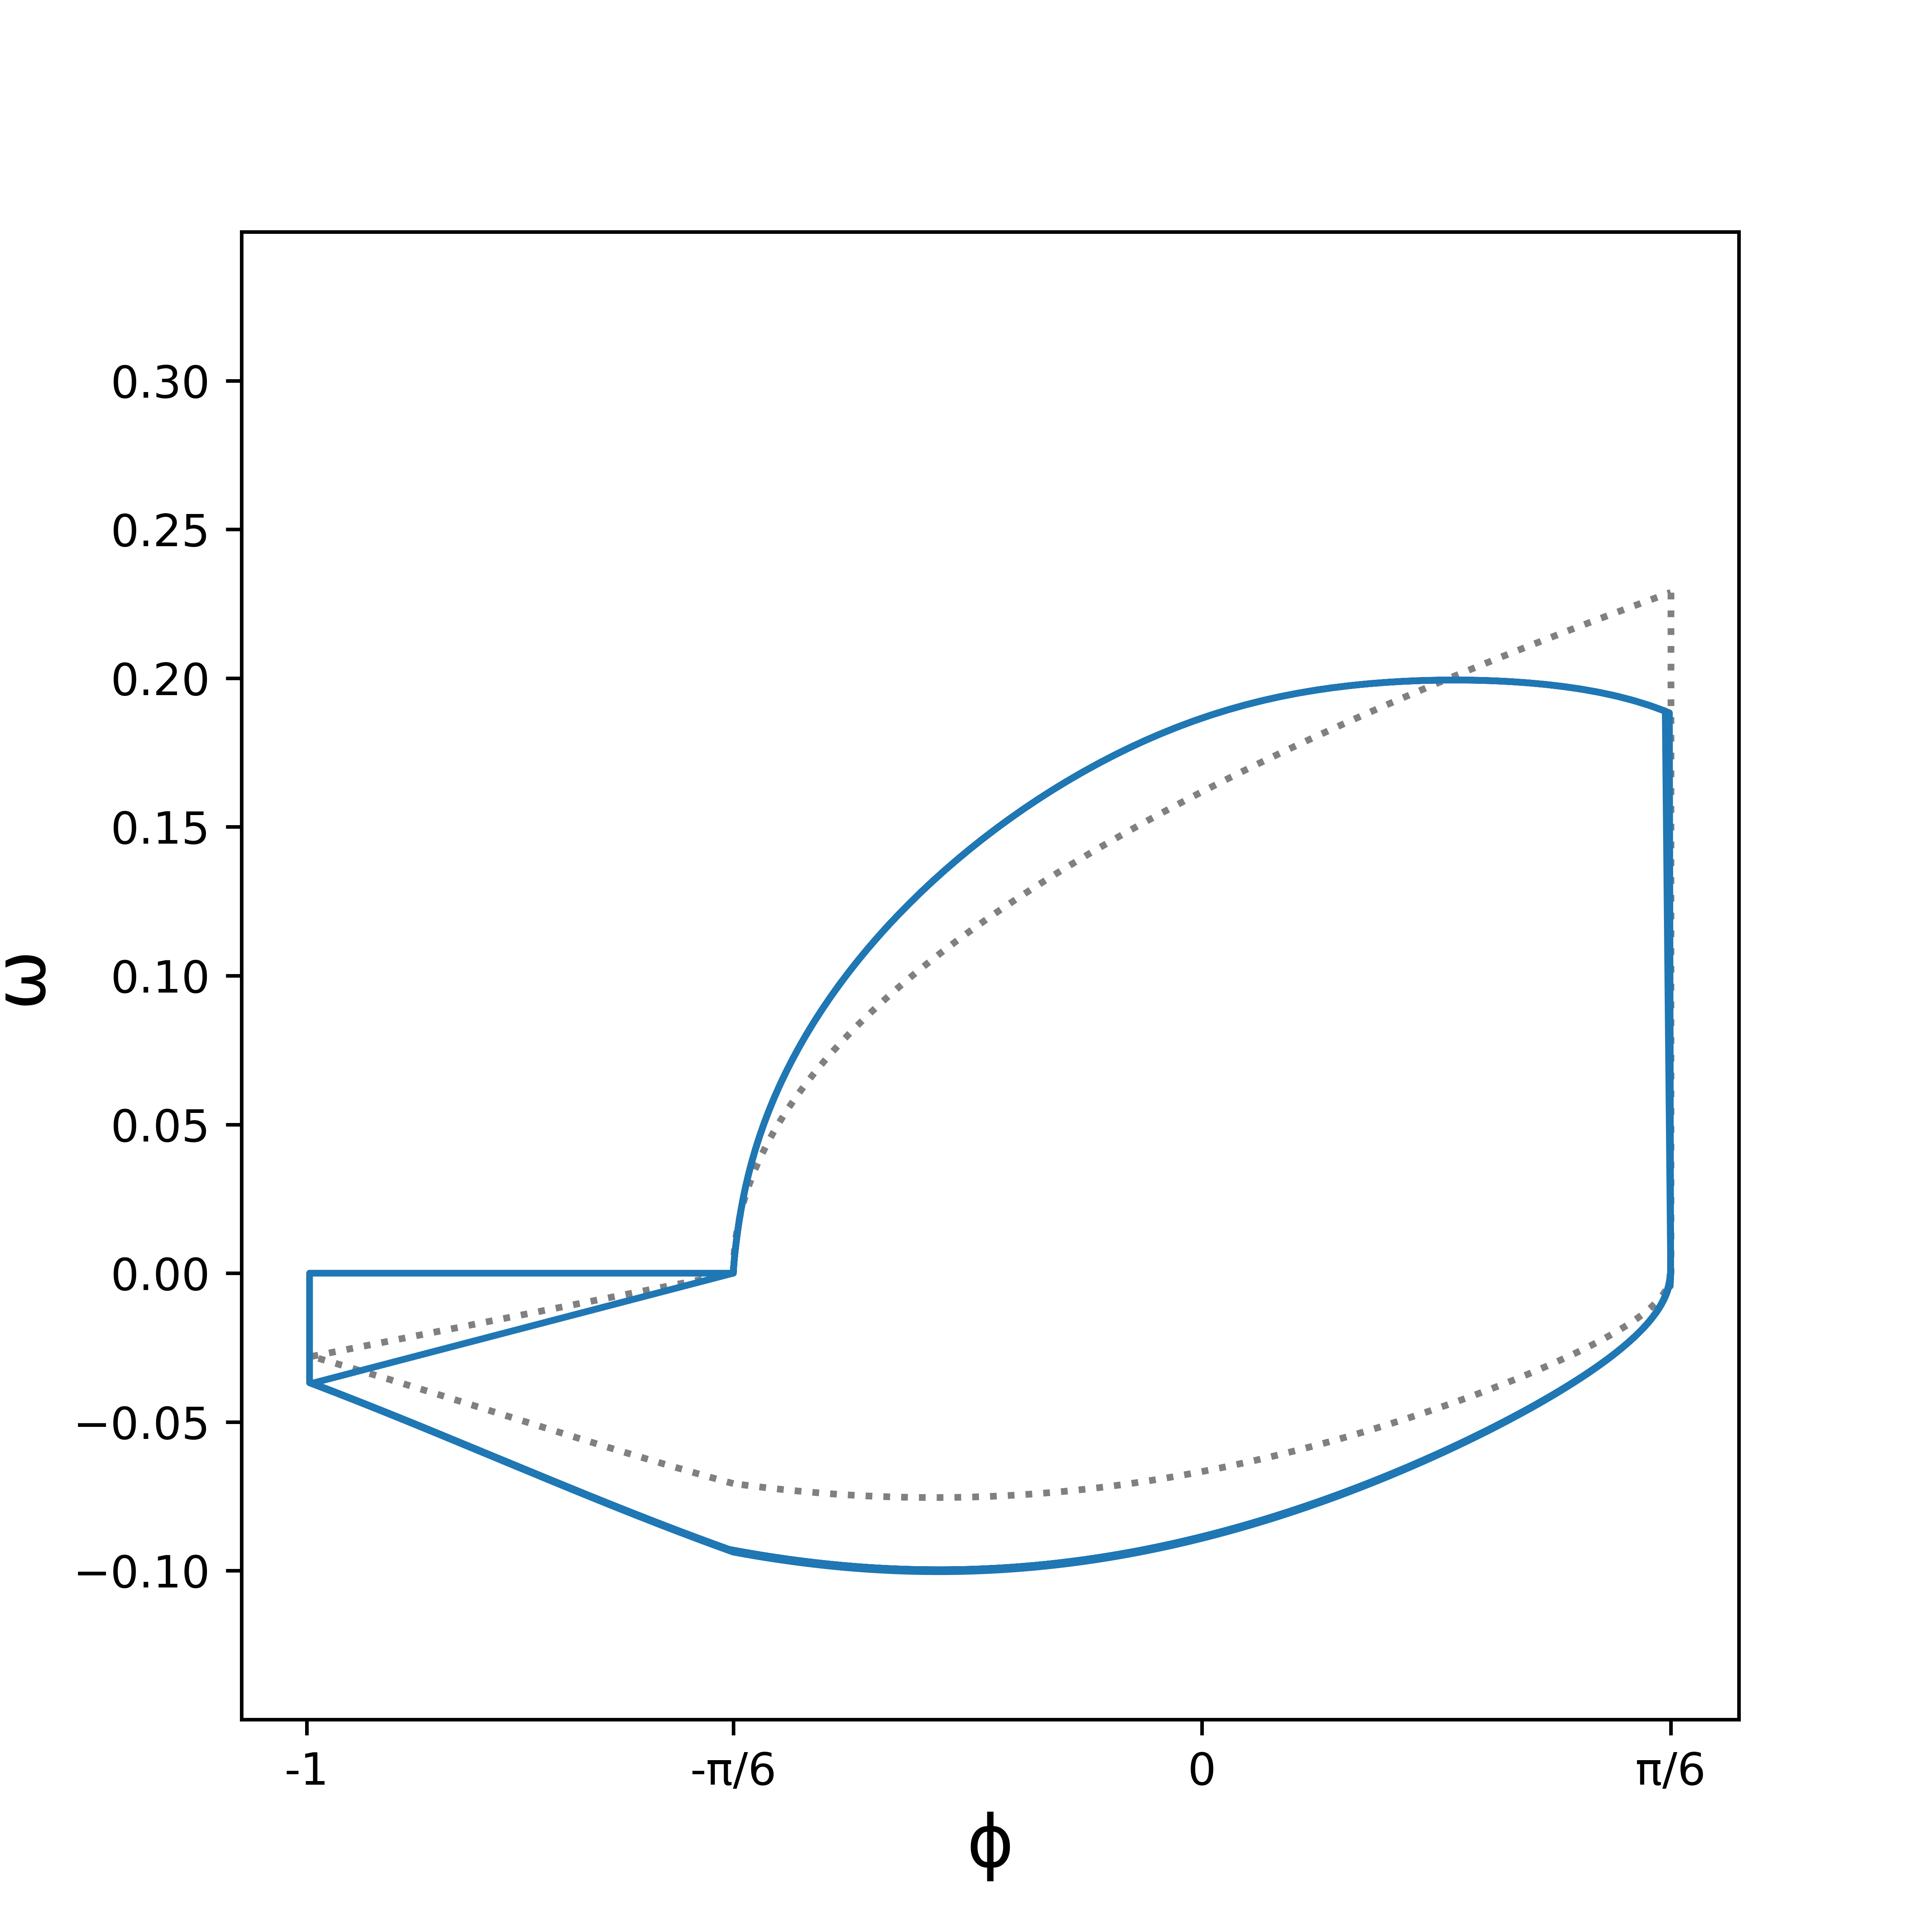
\includegraphics[width=\textwidth]{../plots/trajectory2_126_116.png}
    \caption{}
    \label{fig:DuckPlot2Cheat}
  \end{subfigure}%
  \hspace{-15pt}% Adjust horizontal spacing here
  \begin{subfigure}[b]{0.5\textwidth}
    \vspace{0pt} % Adjust vertical spacing here
    \centering
    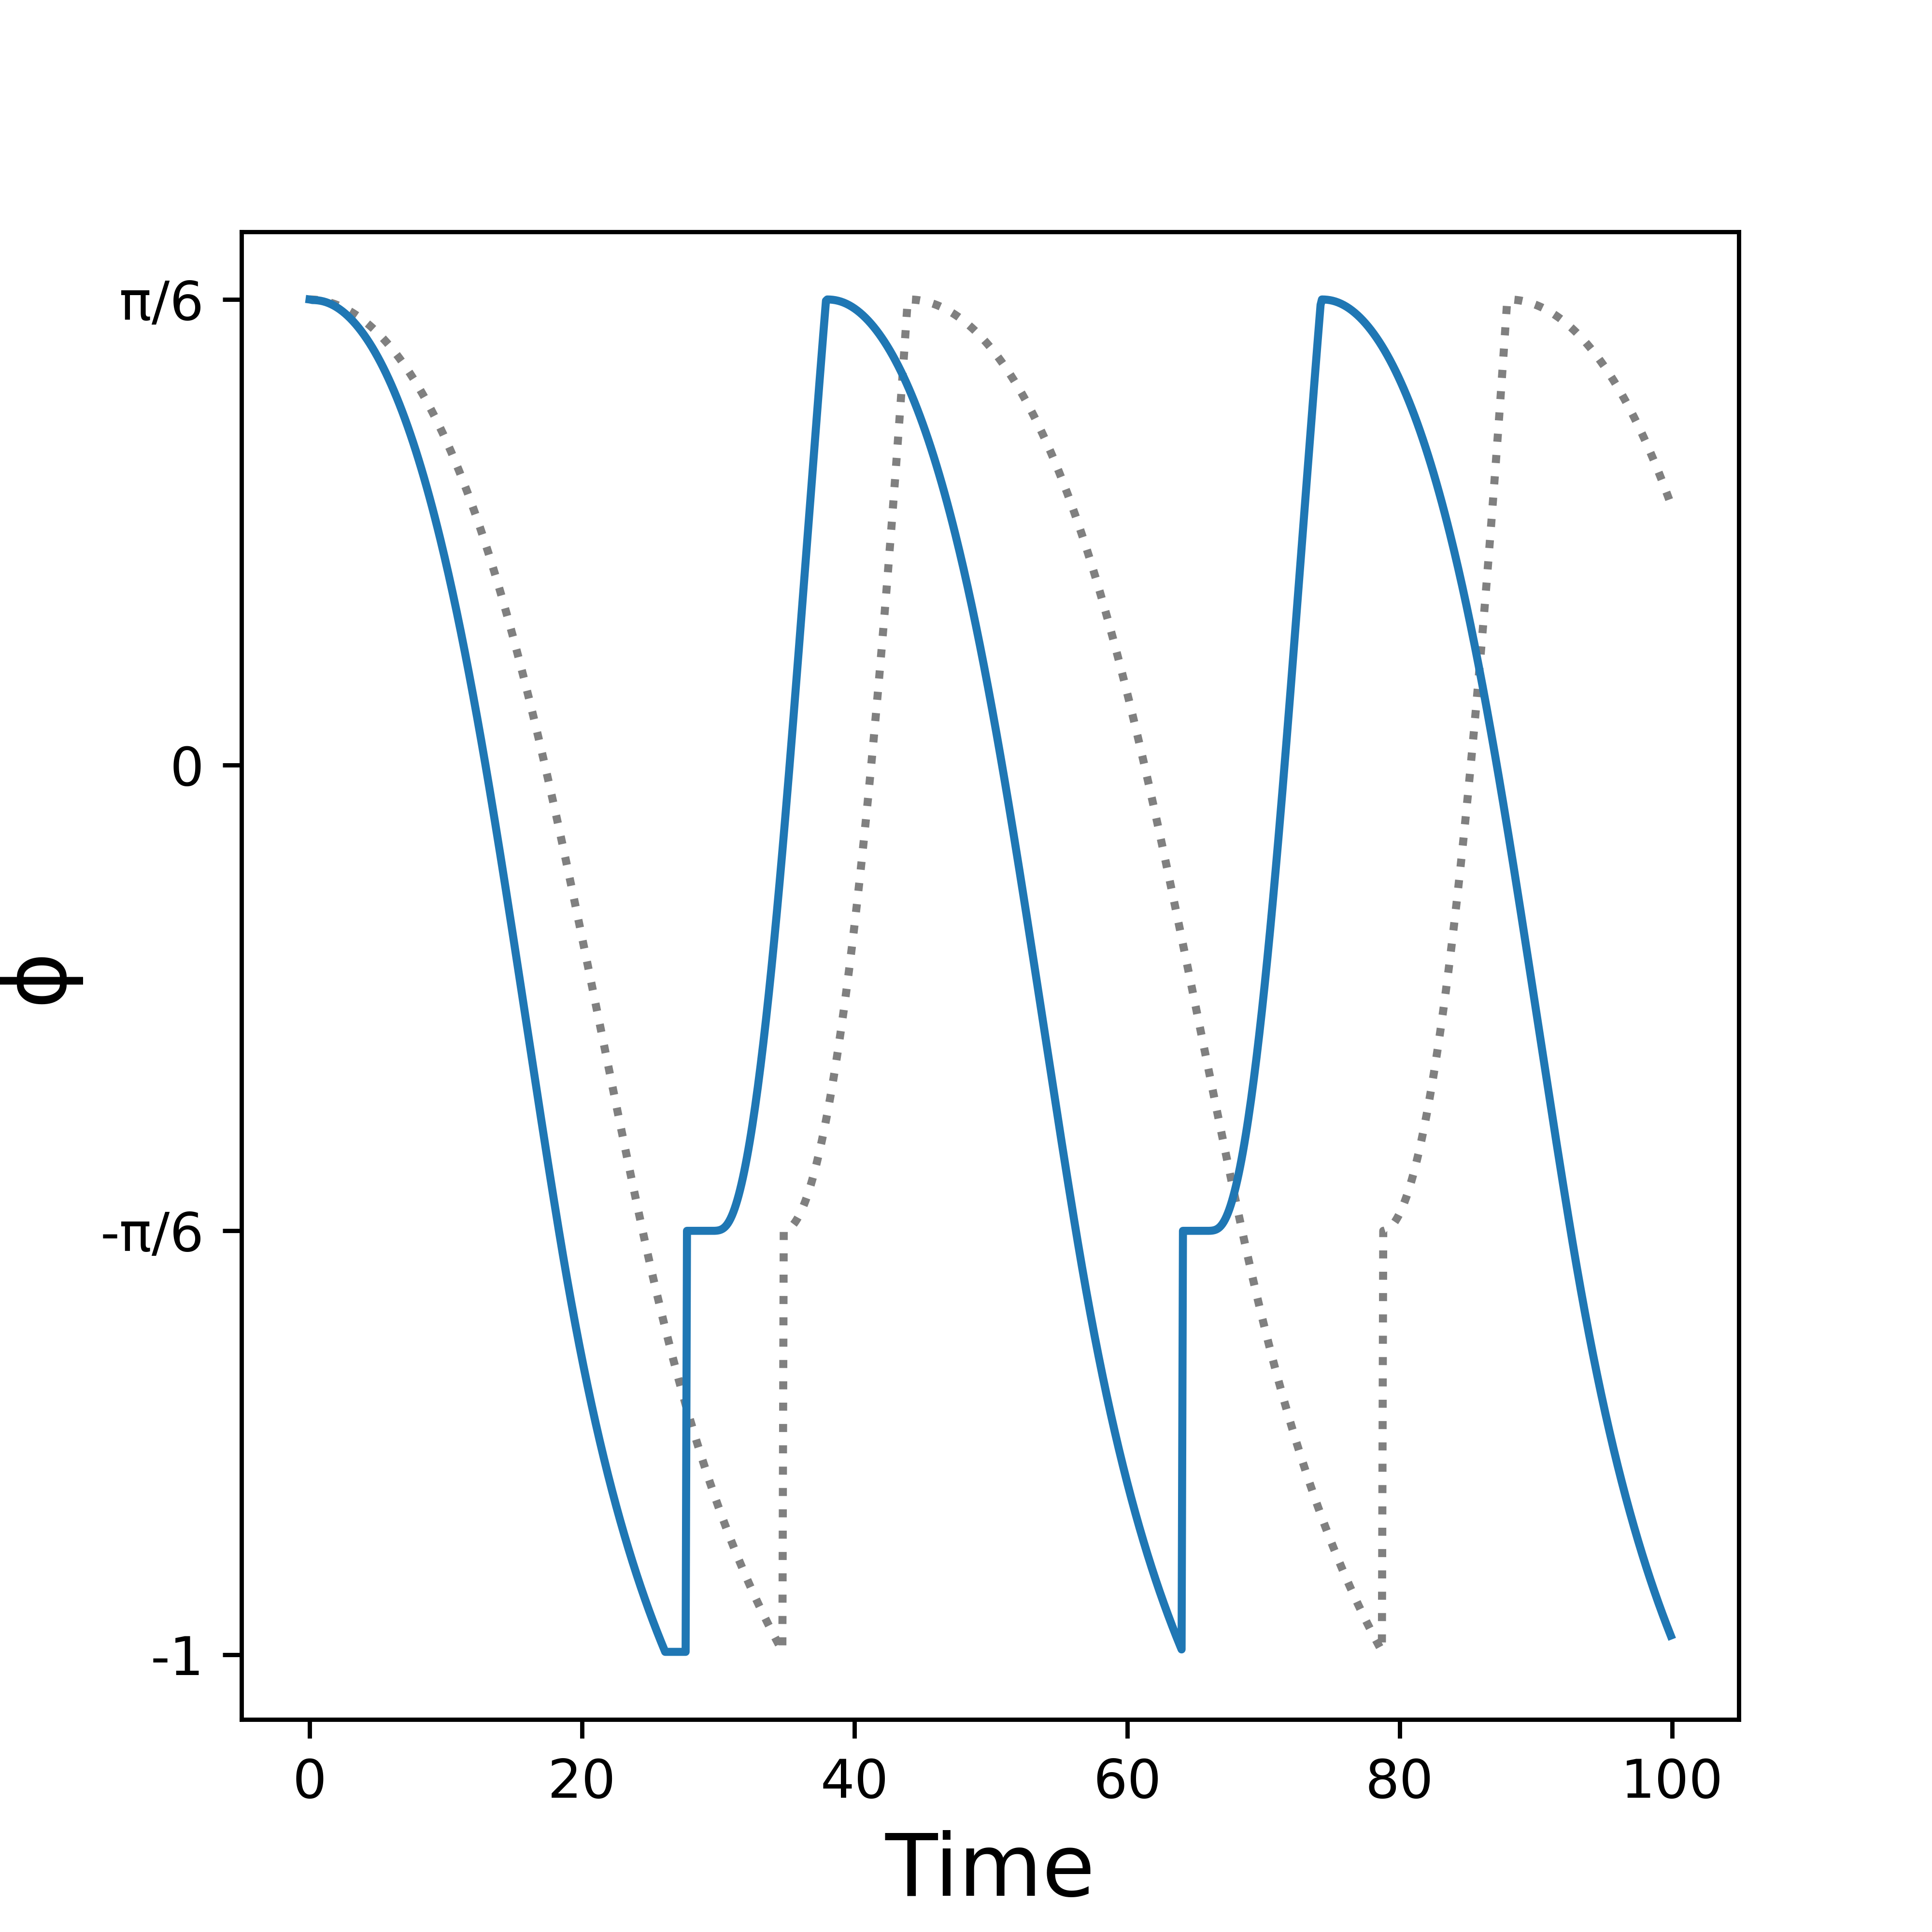
\includegraphics[width=\textwidth]{../plots/angleTime2_126_116.png}
    \caption{}
    \label{fig:AngleTimePlot2Cheat}
  \end{subfigure}
  \caption{Plots of trajectory of most fit "cheater" two neuron agent [[1,1,-1,0,0],[-1,-1,1,0,0]] (blue), where all effectors receive signal from both neurons but do not have any sensory connections, compared with optimal trajectory (grey). (a) Plot of leg trajectories as leg angle \((\phi)\) by leg angle velocity \((\omega)\). (b) Plot of leg angles over time}
  \label{fig:plots2Cheat}
\end{figure} 

To confirm this, I examined the trajectory of a "cheater" agent, one that had the strong motor output of the best agent, but with no sensory connections (see Fig \ref{fig:plots2Cheat}). Like the best agent, the cheater agent was capable of velocities exceeding the optimal step, resulting in faster steps and a overall fitness of ~0.773. Notably, judging from the rounded upper-right curve, the cheater agent was unable to transition from the swing phase to the stance phase efficiently. This indicates that the sensory connections likely also played a role in the remarkably high fitness of the best agent.

\begin{figure}[htbp]
  \centering
  \begin{subfigure}[b]{0.5\textwidth}
    \vspace{0pt} % Adjust vertical spacing here
    \centering
    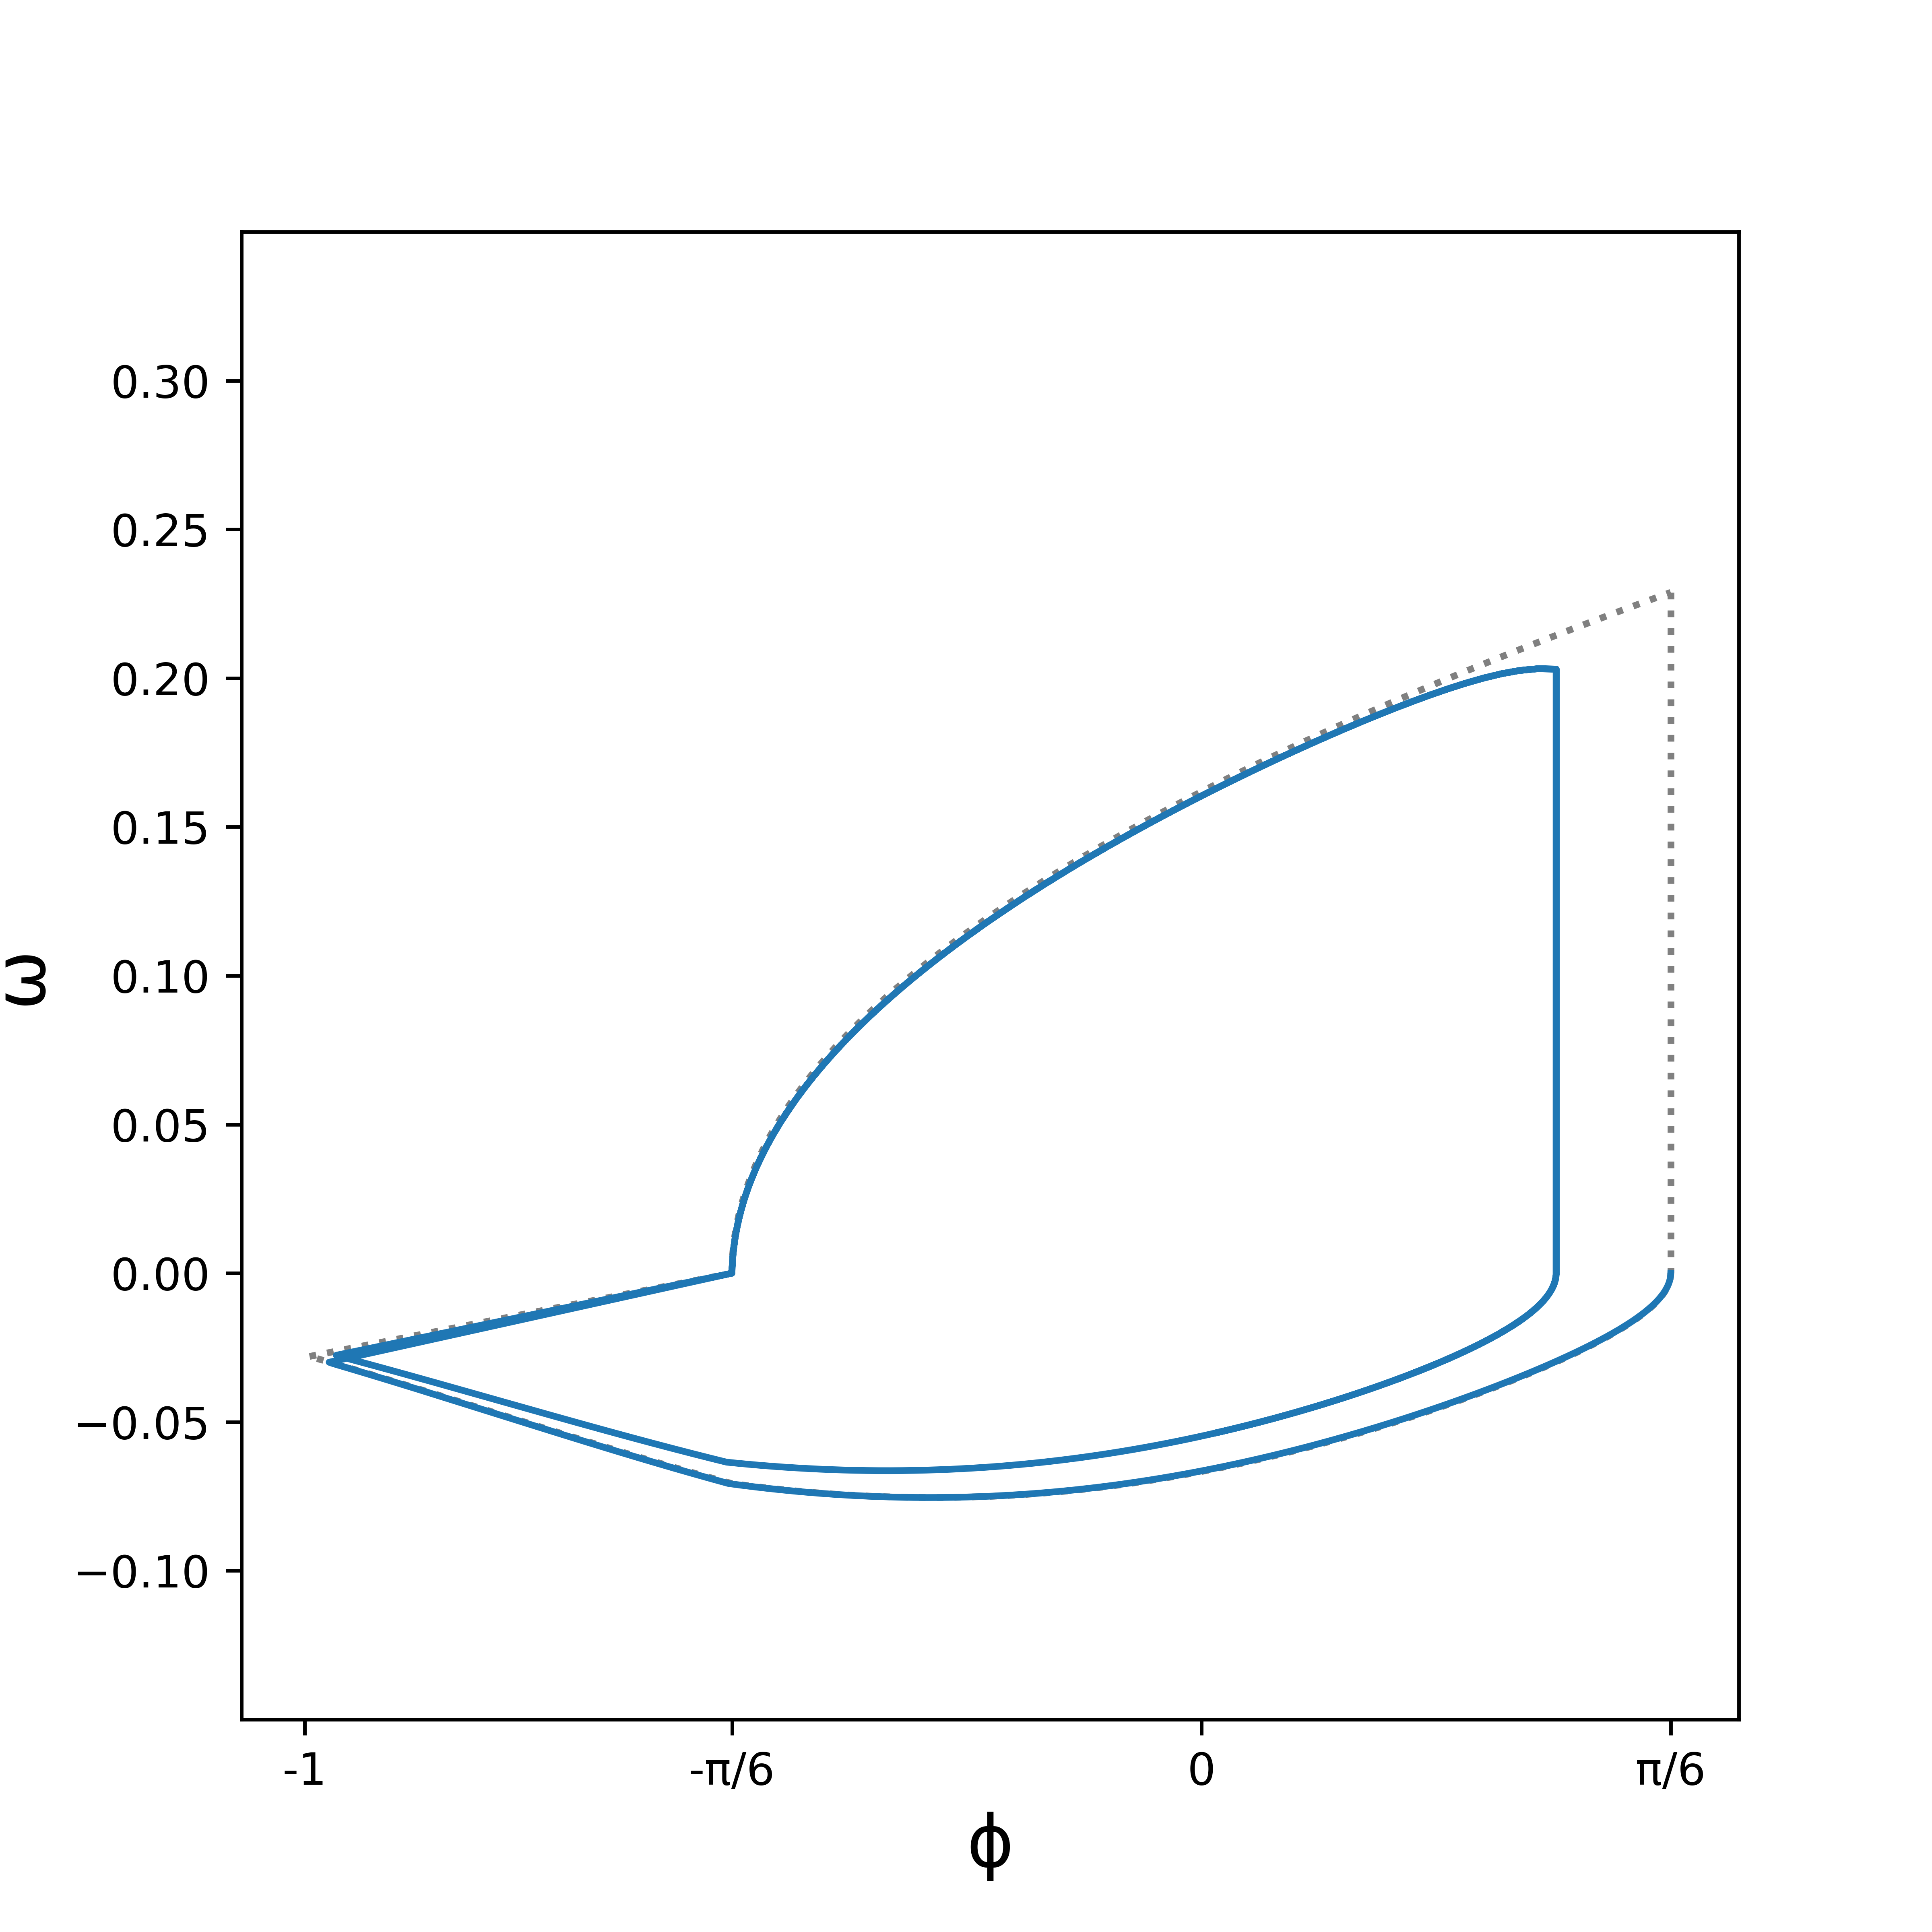
\includegraphics[width=\textwidth]{../plots/trajectory2_233_22.png}
    \caption{}
    \label{fig:DuckPlot2Fair}
  \end{subfigure}%
  \hspace{-15pt}% Adjust horizontal spacing here
  \begin{subfigure}[b]{0.5\textwidth}
    \vspace{0pt} % Adjust vertical spacing here
    \centering
    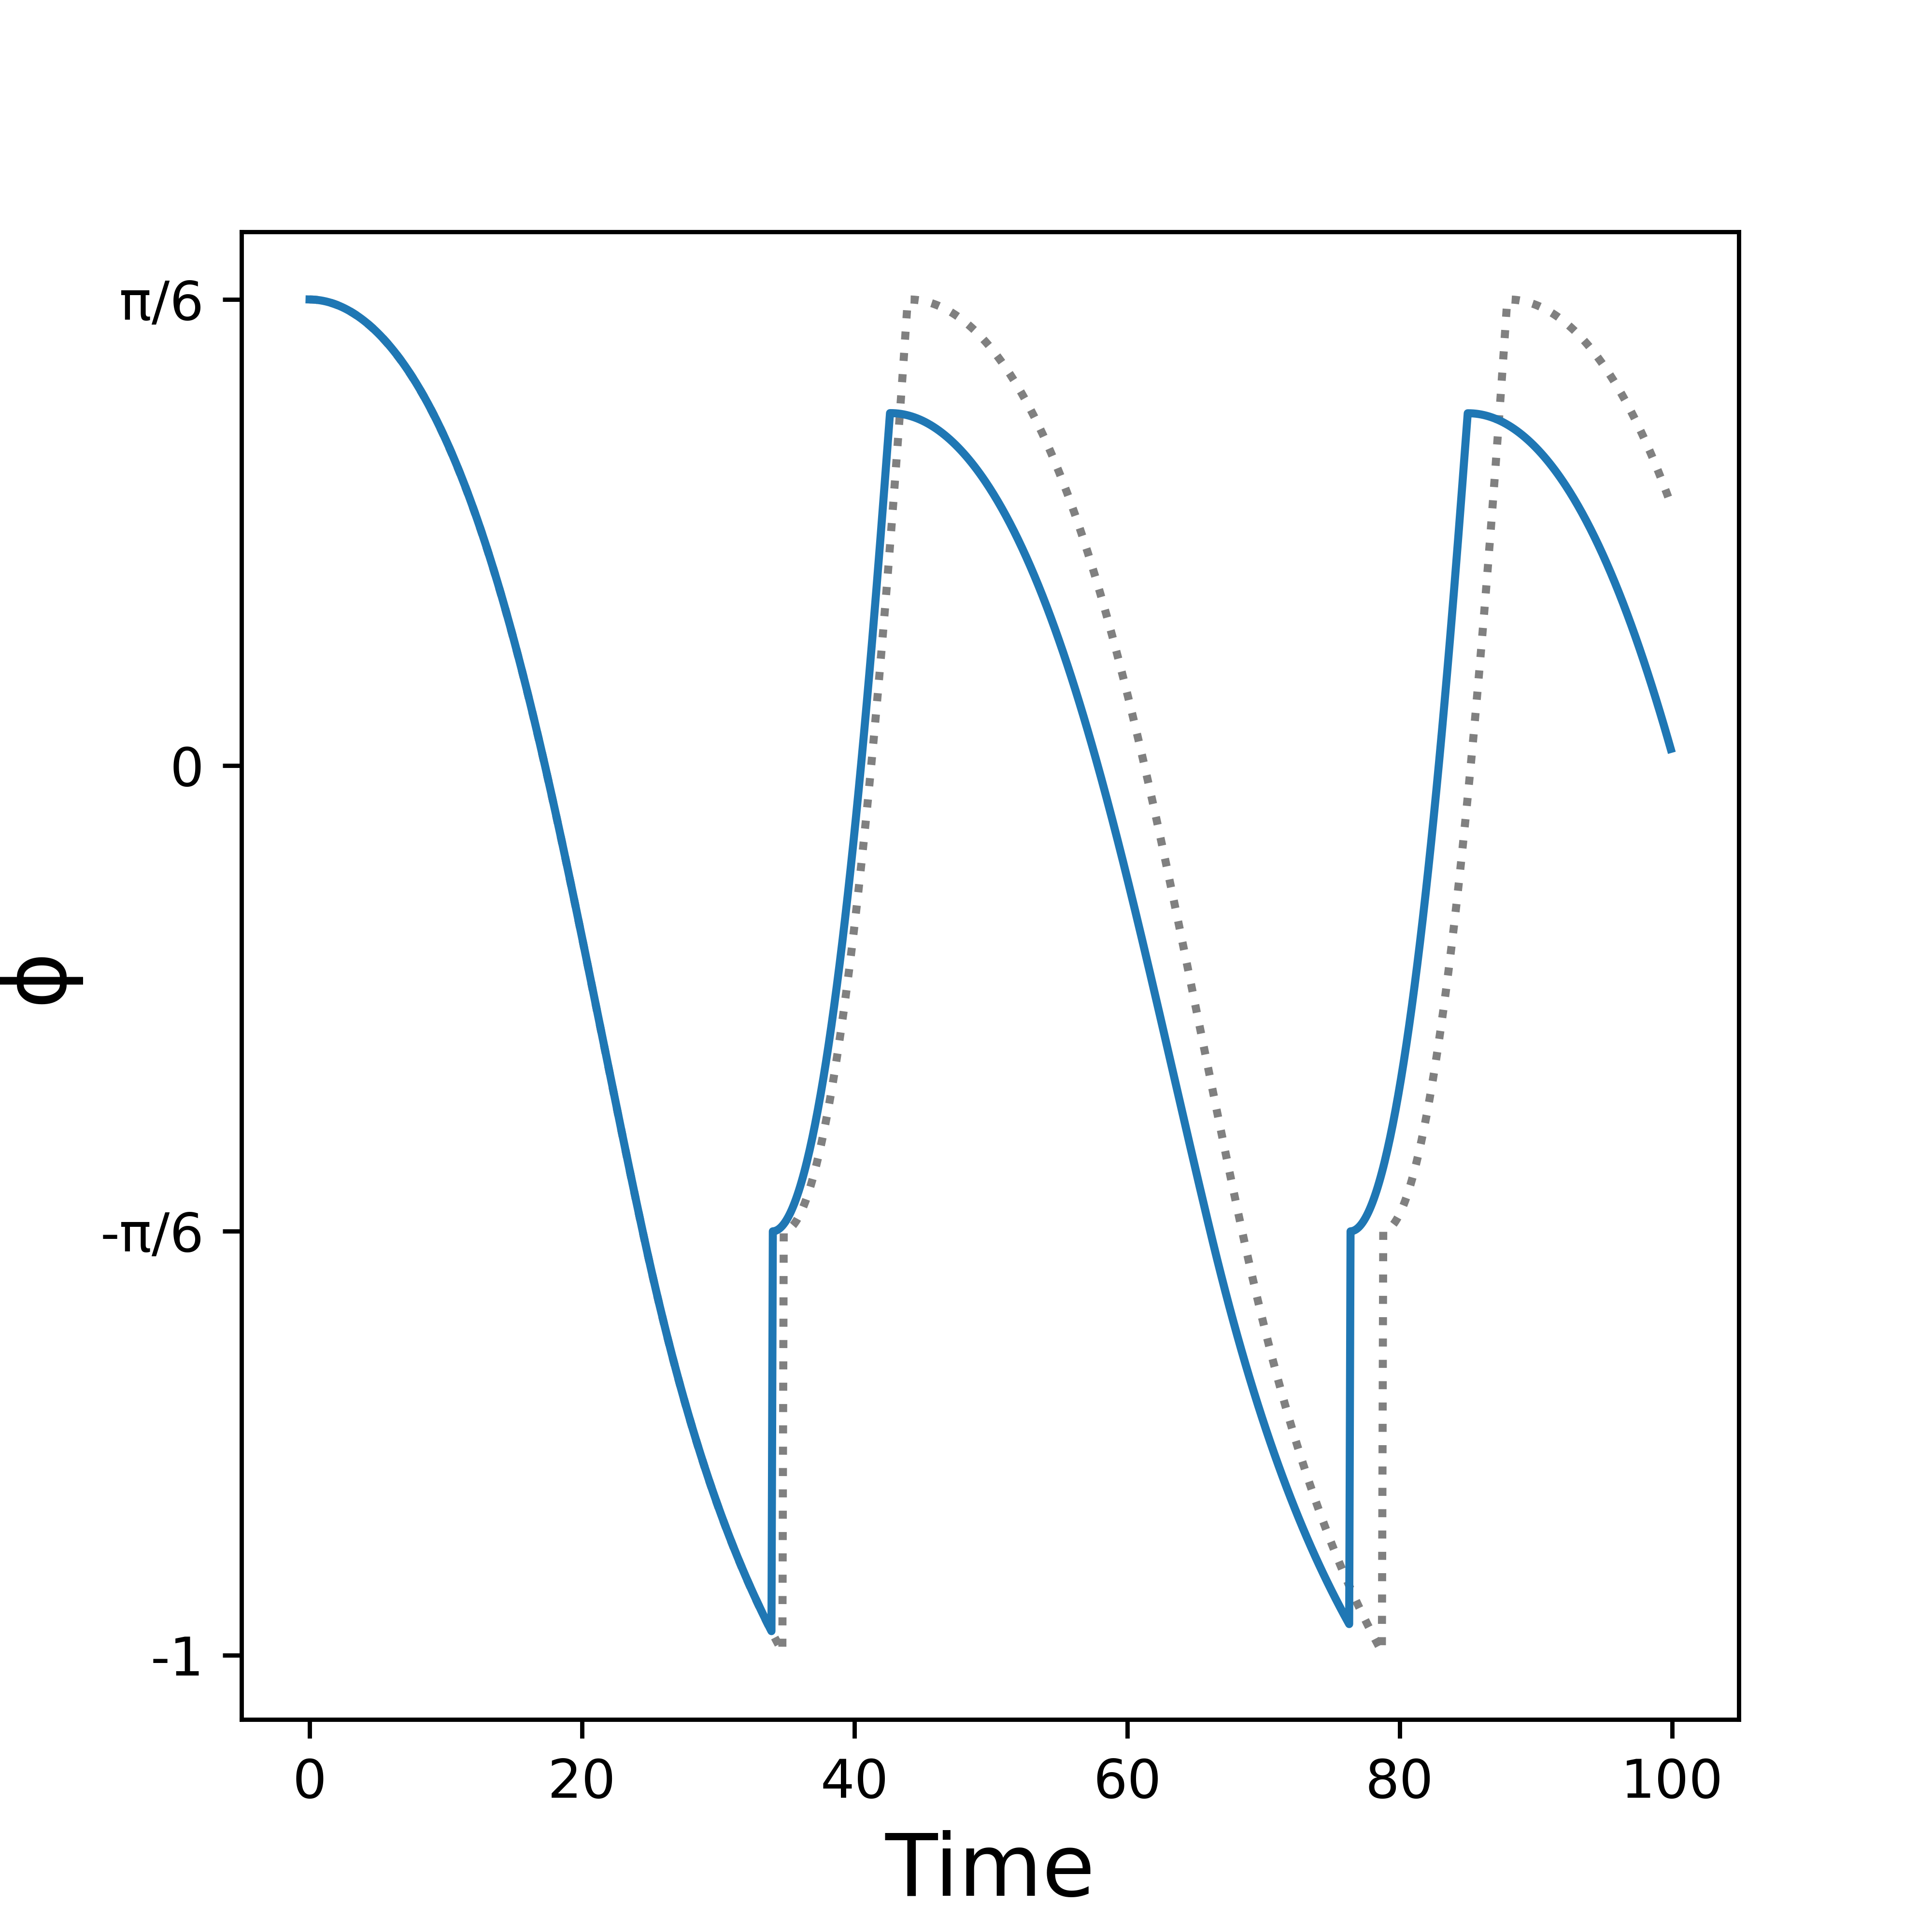
\includegraphics[width=\textwidth]{../plots/angleTime2_233_22.png}
    \caption{}
    \label{fig:AngleTimePlot2Fair}
  \end{subfigure}
  \caption{Plots of trajectory of most fit "fair" two neuron agent [[1,1,0,1,1],[0,0,1,-1,-1]] (blue), where all effectors receive signal from a single neuron, compared with optimal trajectory (grey). (a) Plot of leg trajectories as leg angle \((\phi)\) by leg angle velocity \((\omega)\). (b) Plot of leg angles over time}
  \label{fig:plots2Fair}
\end{figure} 

To better understand the role of the sensory connections, I examined the trajectory of the best agent with the limitation that each effector would only receive output from a single neuron (see Fig \ref{fig:plots2Fair}). This would show how the sensory connections impacted the behavior of the agent without the confounding factor of the effectors receiving output from both neurons. I referred to this agent as the "fair" agent as it did not take advantage of the extra neural output to the effectors and only was able to take advantage of the sensory feedback. Looking at Fig \ref{fig:DuckPlot2Fair}, the trajectory of the fair agent is much worse than what an optimal walker would produce, having the entire trajectory contained inside the range of the optimal step. However, Fig \ref{fig:AngleTimePlot2Fair} paints a different story. The fair agent switches from swing to stance phase early. While this results in a shorter distance traveled every step, the agent is able to take more steps in the same amount of time, resulting in a very slightly higher overall fitness than the optimal walker (~0.622). This fitness advantage is likely sensitive to the length in time of the simulation as well as when the simulation is stopped. If both agents had their fitness calculated during their swing phase, the optimal walker would likely have a higher fitness. However, if both agents had their fitness calculated during their stance phase, the fair agent would likely have a higher fitness. This indicates that the sensory connections are responsible for the sharp transitions between swing to stance in the best agent, contributing to its high fitness.

\section{Conclusion}
% Add your conclusion content here

The results of this study indicate that sensorimotor connections play a significant role in the fitness of a single-legged walker. In both the one and two neurons cases, having a foot effector connection and more forward output than backward output was necessary for movement. For the single neuron CTRNNS, sensory connections were not necessary for movement, but a positive connection to the angle sensor and/or a negative connection to the foot sensor appeared to improve fitness. Some agents were even capable of oscillations in spite of not possessing an central pattern generator. Employing bodily constraints as a means of creating an oscillatory mechanism with the assistance of neural feedback appears to be possible in even simple systems such as this one.

The two neuron CTRNNs were capable of a much greater range of behaviors than the single neuron CTRNNs. With twice as much power to the effectors, the two neuron CTRNNs were capable of reaching a fitness greater than that of an optimal walker. This was possible even when the effectors were limited to a single neuron each, indicating that the sensory connections played a role in the sharp transitions between swing and stance phases, resulting in a higher fitness than an optimal walker. Even with only two neurons, the more complex sensorimotor connections available to these agents allowed for a greater range of behaviors than found in three neuron CTRNNs evolved for the same task \cite{BeerWalker}.

\section{Future Directions}
% Add your conclusion content here
Whether through continuation of the current work or expansion into new ideas, there are many interesting future directions for this work. The increased fitness of the single neuron CTRNN agent with a negative angle connection remains a mystery. Further examination of how fitness and overall distance are calculated may provide insight into why this is the case. Given that the "optimal" walker was not very optimal for these sets of experiments, it may be interesting to calculate what the trajectory of this new optimal walker would look like.

Given the high fitness scores capable of the two neuron model, it would be interesting to explore the sensorimotor couplings of a three neuron model. This may provide more possibilities for an interneuron capable of improving performance, as opposed to the one and two neuron cases where all neurons needed to have sensorimotor connections to have maximum fitness. It may also prove interesting to model these neurons such that they learn which connections to have to improve fitness from sensory feedback, using a reinforcement learning approach. Finally, further examination of the dynamics of the leg swing would be another interesting direction, as it may expand our overall understanding of the interplay of the various parameters in the system.



\section{Code Availability}
All code used in this project is available at \texttt{https://github.com/Zach-Attach/SingleLeggedWalker/tree/pairing}.

% Import references from references.tex
\pagebreak
\bibliography{ref}
\bibliographystyle{apalike}

\end{document}
